\chapter{Structured Recurrent Memory: Log-Linear Attention, Mixture-of-Memories, Mamba-3}\label{ch:structured}

A linear-attention layer or a state space model keeps its whole memory of the past in one
matrix per head. \Cref{ch:linear} showed how to train such a layer in parallel and decode it
in constant time and memory, and \cref{ch:delta,ch:expressive} showed how to make the
\emph{write} into that matrix smarter: forget with a gate, overwrite with the delta rule, or
transform the state with a richer matrix. None of those changes how much the memory can
hold. A $d_v \times d_k$ matrix can store at most $d_k$ key--value associations without
crosstalk, no matter how cleverly it is written. Once a sequence holds more facts than that,
new writes interfere with old ones.

This chapter studies three 2025--2026 designs that change how recurrent memory
\emph{capacity is organized}. Log-Linear Attention~\citep{guo2025loglinear} replaces the
single state with a small set of states, one per level of a Fenwick tree over the past, so
the number of states grows as $\log T$ and recent tokens are kept at a finer resolution than
distant ones. Mixture-of-Memories (MoM)~\citep{du2025mom} keeps several independent states
and lets a learned router decide which of them each token is written to, so unrelated
content does not share a matrix. Mamba-3~\citep{lahoti2026mamba3} keeps one state but makes
better use of it: a more accurate (trapezoidal) discretization, complex-valued (rotating)
state transitions that are implemented as data-dependent rotary embeddings, and
multi-input multi-output (MIMO) updates that write a rank-$R$ matrix per step at almost no
extra decoding cost.

\Cref{sec:c07-background} recaps the single-state picture and quantifies interference.
\Cref{sec:c07-loglinear,sec:c07-mom,sec:c07-mamba3} treat the three systems, each with its
mathematics, algorithms, a walk through the official code and a from-scratch reference
implementation. \Cref{sec:c07-comparison} compares them.

% =====================================================================
\section{Background: how much can one recurrent state hold?}\label{sec:c07-background}
% =====================================================================

\subsection{One state, one mask}\label{sec:c07-onestate}

We work with one head and drop the head index. Gated linear attention, the common core of
Mamba-2, GLA and their relatives (\cref{ch:linear}), keeps a matrix state
$\mS_t \in \R^{d_v \times d_k}$ and updates and reads it as
\begin{equation}\label{eq:c07-gla}
  \mS_t = \alpha_t \mS_{t-1} + \vv_t \vk_t\T, \qquad \vo_t = \mS_t \vq_t ,
\end{equation}
with a decay $\alpha_t \in (0,1]$ and $\mS_0 = \bm{0}$. Unrolling the recursion,
\begin{equation}\label{eq:c07-unroll}
  \mS_t = \sum_{s=1}^{t} \Gamma_{ts}\, \vv_s \vk_s\T,
  \qquad \Gamma_{ts} \defeq \prod_{r=s+1}^{t} \alpha_r \quad (\Gamma_{tt} = 1),
\end{equation}
so $\vo_t = \sum_{s \le t} \Gamma_{ts}\, (\vk_s\T \vq_t)\, \vv_s$. Stacking the outputs as
rows of $\mO \in \R^{T \times d_v}$ gives the \emph{parallel form}
\begin{equation}\label{eq:c07-parallel}
  \mO = \bigl(\mQ\mK\T \had \bm{\Gamma}\bigr) \mV ,
\end{equation}
where $\bm{\Gamma} \in \R^{T\times T}$ is lower triangular with entries $\Gamma_{ts}$ for
$s \le t$. Mamba-2 is exactly this form with $\vq_t = \vec{C}_t$, $\vk_t = \vec{B}_t$,
$\vv_t = \Delta_t \vx_t$ and $\alpha_t = \exp(\Delta_t A)$~\citep{dao2024ssd}.

The mask $\bm{\Gamma}$ is highly structured. Let $c_t = \prod_{r \le t}\alpha_r$; then
$\Gamma_{ts} = c_t / c_s$ for $s \le t$. Any block of $\bm{\Gamma}$ that lies entirely below
the diagonal is therefore an outer product $(c_t)_t (1/c_s)_s\T$, a rank-one matrix. Matrices
with this property are called \emph{1-semiseparable}. The low rank of every below-diagonal
block is what makes the chunkwise algorithm of \cref{ch:linear} possible: split the sequence
into chunks of $C$ tokens; everything that chunk $[i]$ needs from earlier chunks passes
through one matrix, the state $\mS_{[i-1]}$ at the end of the previous chunk,
\begin{equation}\label{eq:c07-chunk}
  \mO_{[i]} = \bigl(\mQ_{[i]}\mK_{[i]}\T \had \bm{\Gamma}_{[i]}\bigr)\mV_{[i]}
            + \diag\bigl(\vg_{[i]}\bigr)\, \mQ_{[i]}\mS_{[i-1]}\T ,
\end{equation}
where $\bm{\Gamma}_{[i]}$ is the $C \times C$ diagonal block of $\bm{\Gamma}$ and
$\vg_{[i]}$ holds the decay from the start of the chunk to each of its positions. Training
costs $\bigO(TC(d_k+d_v) + T d_k d_v)$ per head and decoding costs
$\bigO(d_k d_v)$ time and memory per token.

\subsection{Interference: what a single matrix can store}\label{sec:c07-interference}

Ignore decay for a moment and write $n$ key--value pairs into one state,
$\mS = \sum_{i=1}^{n} \vv_i \vk_i\T$. Reading with the $j$-th key gives
\begin{equation}\label{eq:c07-crosstalk}
  \mS \vk_j = \norm{\vk_j}^2 \vv_j + \underbrace{\sum_{i \ne j} (\vk_i\T \vk_j)\, \vv_i}_{\text{crosstalk}} .
\end{equation}
If the keys are orthonormal the crosstalk vanishes and every value is recalled exactly. But
$\R^{d_k}$ contains at most $d_k$ orthonormal vectors.

\begin{proposition}\label{prop:c07-capacity}
If $n > d_k$, no matrix $\mS \in \R^{d_v \times d_k}$ can satisfy $\mS\vk_j = \vv_j$ for all
$j$ and all choices of the values $\vv_1, \dots, \vv_n$.
\end{proposition}
\begin{proof}
With $n > d_k$ the keys are linearly dependent, so some key is a combination of the others,
$\vk_j = \sum_{i \ne j} c_i \vk_i$. Any linear read-out then satisfies
$\mS\vk_j = \sum_{i\ne j} c_i \mS\vk_i$. If all other values were recalled exactly, the
$j$-th read would be forced to equal $\sum_{i \ne j} c_i \vv_i$, which differs from $\vv_j$
for most choices of $\vv_j$.
\end{proof}

How large is the crosstalk for random keys? Let the entries of $\vk_i$ be independent with
mean $0$ and variance $1/d_k$ (so $\E\norm{\vk_i}^2 = 1$), and let the values have independent
unit-variance coordinates. For $i \ne j$,
$\E[(\vk_i\T\vk_j)^2] = \sum_{a=1}^{d_k} \E[k_{ia}^2]\E[k_{ja}^2] = d_k \cdot d_k^{-2} = 1/d_k$,
and the $n-1$ crosstalk terms are uncorrelated, so each coordinate of the crosstalk has
\begin{equation}\label{eq:c07-crosstalk-var}
  \E\bigl[\text{crosstalk}^2\bigr] = \frac{n-1}{d_k}.
\end{equation}
The signal has unit size, so retrieval degrades once $n$ approaches $d_k$. A quick Monte
Carlo check with $d_k = 64$ (in our scratch scripts) gives $1.05$, $3.94$ and $17.2$ for
$n = 64$, $256$ and $1024$, against the prediction $0.98$, $3.98$ and $15.98$.

\begin{example}[Four facts in a two-dimensional key space]\label{ex:c07-four}
Let $d_k = 2$ and store four pairs with keys $\ve_1, \ve_2, \vec{f}_1 = (\ve_1+\ve_2)/\sqrt2,
\vec{f}_2 = (\ve_1 - \ve_2)/\sqrt2$ and one-hot values $\ve_1,\dots,\ve_4 \in \R^4$. Then
$\mS\ve_1 = (1,\, 0,\, 0.707,\, 0.707)\T$ instead of $(1,0,0,0)\T$, and every one of the four reads
is off by exactly $1$ in Euclidean norm. If instead the first two pairs go to one matrix and
the last two to another, each matrix holds an orthonormal key set and all four reads are
exact. This is the idea behind MoM in \cref{sec:c07-mom}.
\end{example}

Gating and the delta rule (\cref{ch:linear,ch:delta}) manage interference by forgetting or by
overwriting the value stored under a key. They do not change the fact that the whole past
shares one $d_v\times d_k$ matrix. \Cref{tab:c07-routes} lists the three ways this chapter
reorganizes that capacity.

\begin{table}[t]
\centering\small
\caption{Three ways to reorganize the capacity of recurrent memory.}
\label{tab:c07-routes}
\begin{tabularx}{\textwidth}{@{}l l l X@{}}
\toprule
Route & System & States per head & What decides where a token is stored \\
\midrule
More states over time & Log-Linear Attention & $\le \lceil\log_2 T\rceil + 1$ & Its position: a Fenwick-tree partition of the past \\
More states over content & MoM & $M$ (plus one shared) & Its content: a learned top-$k$ router \\
A better single state & Mamba-3 & $1$ & Not applicable; the transition and the write become richer \\
\bottomrule
\end{tabularx}
\end{table}

% =====================================================================
\section{Log-Linear Attention}\label{sec:c07-loglinear}
% =====================================================================

\subsection{Motivation}

Softmax attention and linear attention sit at two extremes. Softmax attention keeps every
past token at full resolution in its KV cache, which grows linearly with $T$, and pays
$\bigO(T)$ per decoded token. Linear attention keeps a constant-size state and pays
$\bigO(1)$, but everything in the past is blended into one matrix. Log-linear
attention~\citep{guo2025loglinear} takes the middle road: keep $\bigO(\log T)$ matrices, each
summarizing one segment of the past, with short segments for recent tokens and long
segments for old ones. The query reads every segment through its own data-dependent weight
$\lambda$, so the model can, for example, attend sharply to the recent past while still
reading a coarse summary of the distant past. Training costs $\bigO(T\log T)$ and decoding
costs $\bigO(\log T)$ time and memory per token. The construction is a general recipe: any
linear attention whose mask is semiseparable, such as Mamba-2 or Gated DeltaNet, can be made
log-linear.

\begin{taxonomy}
\textbf{Representation:} implicit; the states are produced by the forward pass.
\textbf{Update dynamics:} online; every token is written at inference time.
\textbf{Persistence:} long-term within a sequence; Table~I of \citet{zhoubian2026memory} lists it
as Online / Long-Term with the paradigm ``Logarithmic Hierarchy of Recurrent States''.
\textbf{Update rule (Table~II):} state-transition updates. The survey describes it as
distributing updates across hierarchical states, ``preserving recent information at finer
resolution and distant history in coarser summaries'', a middle ground between
constant-state linear attention and token-wise KV storage (\S III-C).
\end{taxonomy}

\subsection{Fenwick trees from scratch}\label{sec:c07-fenwick}

A Fenwick tree, or binary indexed tree~\citep{c07-fenwick1994}, answers prefix-sum queries
over an array that keeps changing. Number the positions from $1$ and let
$\operatorname{lowbit}(t) = t \mathbin{\&} (-t)$ be the value of the lowest set bit of $t$
(for $t = 12 = 1100_2$, $\operatorname{lowbit}(t) = 4$). The tree stores, at node $t$, the sum
over the range $(t - \operatorname{lowbit}(t),\, t]$. A prefix $[1, t]$ is the disjoint union
of such ranges, obtained by repeatedly stripping the lowest set bit:
\[
  [1, 13] = (12, 13] \cup (8, 12] \cup (0, 8], \qquad 13 = 1101_2 \to 1100_2 \to 1000_2 \to 0 .
\]
There is one range per set bit of $t$, so at most $\lfloor \log_2 t\rfloor + 1$ ranges, and
their lengths are the powers of two in the binary expansion of $t$, \emph{smallest nearest to
$t$}. That last property is exactly what a memory wants: fine resolution for the recent past,
coarse resolution for the distant past.

\paragraph{The partition used by log-linear attention.}
From here on we number positions from $0$, as the code does. For query position $t$, the
prefix $[0, t]$ is split into the token $t$ itself (level $0$) and the Fenwick decomposition
of the $t$ tokens before it. A compact closed form for the level of each source token turns
out to be the bit length of an exclusive-or.

\begin{definition}[Fenwick level]\label{def:c07-level}
For $0 \le s \le t$ let
\[
  \ell(t,s) \defeq \begin{cases} 0 & s = t, \\ \operatorname{bitlen}(t \oplus s) = 1 + \lfloor \log_2 (t\oplus s)\rfloor & s < t, \end{cases}
\]
where $\oplus$ is bitwise exclusive-or and $\operatorname{bitlen}(n)$ is the number of binary
digits of $n$. The \emph{bucket} of level $\ell$ seen by query $t$ is
$\mathcal{B}_t^{(\ell)} = \{ s \le t : \ell(t,s) = \ell \}$.
\end{definition}

\begin{proposition}[Fenwick partition]\label{prop:c07-fenwick}
Fix $t \ge 0$. For $\ell \ge 1$ the bucket $\mathcal{B}_t^{(\ell)}$ is non-empty if and only if
bit $\ell-1$ of $t$ is $1$. In that case it is the interval
$[\bar t_\ell - 2^{\ell-1},\, \bar t_\ell)$ with $\bar t_\ell = t - (t \bmod 2^{\ell-1})$, of size
$2^{\ell-1}$. Consequently: (i) every $s \in [0,t]$ lies in exactly one bucket; (ii) there are
$\operatorname{popcount}(t) + 1 \le \lfloor\log_2 t\rfloor + 2$ non-empty buckets; (iii) for
$t < T$, all levels lie in $\{0, 1, \dots, \lceil \log_2 T\rceil\}$.
\end{proposition}
\begin{proof}
Take $s < t$ and let $b$ be the highest bit in which $s$ and $t$ differ. Because $s < t$, $t$
has a $1$ and $s$ a $0$ in bit $b$, and they agree on all bits above $b$; hence
$\ell(t,s) = b+1$. Conversely, the integers that agree with $t$ above bit $b$, have a $0$ in
bit $b$ and arbitrary lower bits are exactly the $2^b$ consecutive integers
$[\bar t_{b+1} - 2^b, \bar t_{b+1})$: $\bar t_{b+1}$ is $t$ with its lowest $b$ bits cleared,
which still has bit $b$ set, and subtracting $2^b$ clears that bit. Such integers exist only
if bit $b$ of $t$ is $1$. This proves the interval description with $\ell = b+1$.
(i) holds because $\ell(t,s)$ is a function of $s$: each source gets exactly one level.
(ii) counts one bucket per set bit plus the level-$0$ bucket $\{t\}$. For (iii), $s, t < T
\le 2^{\lceil\log_2 T\rceil}$, so $t\oplus s < 2^{\lceil\log_2 T\rceil}$ and its bit length is at
most $\lceil \log_2 T\rceil$.
\end{proof}

For $t = 13 = 1101_2$: $\mathcal{B}^{(0)} = \{13\}$, $\mathcal{B}^{(1)} = \{12\}$,
$\mathcal{B}^{(2)} = \emptyset$ (bit~1 of $13$ is $0$), $\mathcal{B}^{(3)} = \{8,\dots,11\}$ and
$\mathcal{B}^{(4)} = \{0,\dots,7\}$, as drawn in \cref{fig:c07-fenwick}. With $T = 16384$
there are $\lceil\log_2 T\rceil+1 = 15$ levels, the value the official code uses. The code
computes the same levels with a recursion (subtract the largest power of two not exceeding
$t$ from both $t$ and $s$ until $s$ falls below it); \cref{ex:c07-fenwick} asks you to show
the two definitions agree.

\begin{figure}[t]
\centering
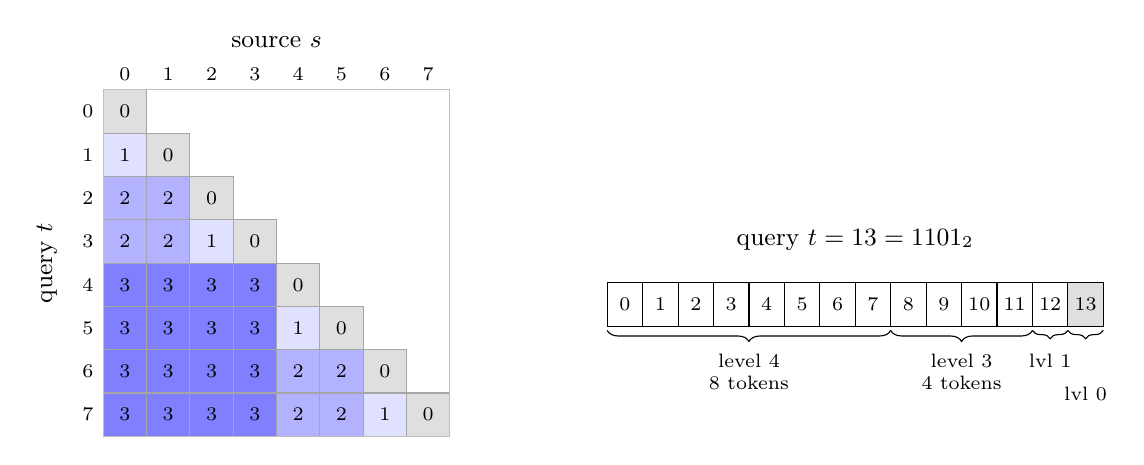
\begin{tikzpicture}[x=0.55cm,y=0.55cm]
  % left: level matrix for T = 8
  \foreach \t/\s/\l/\col in {0/0/0/gray!25,1/0/1/blue!12,1/1/0/gray!25,2/0/2/blue!30,2/1/2/blue!30,2/2/0/gray!25,
    3/0/2/blue!30,3/1/2/blue!30,3/2/1/blue!12,3/3/0/gray!25,4/0/3/blue!50,4/1/3/blue!50,
    4/2/3/blue!50,4/3/3/blue!50,4/4/0/gray!25,5/0/3/blue!50,5/1/3/blue!50,5/2/3/blue!50,
    5/3/3/blue!50,5/4/1/blue!12,5/5/0/gray!25,6/0/3/blue!50,6/1/3/blue!50,6/2/3/blue!50,
    6/3/3/blue!50,6/4/2/blue!30,6/5/2/blue!30,6/6/0/gray!25,7/0/3/blue!50,7/1/3/blue!50,
    7/2/3/blue!50,7/3/3/blue!50,7/4/2/blue!30,7/5/2/blue!30,7/6/1/blue!12,7/7/0/gray!25}
  {
    \fill[\col] (\s,-\t) rectangle ++(1,-1);
    \draw[gray!70] (\s,-\t) rectangle ++(1,-1);
    \node[font=\scriptsize] at (\s+0.5,-\t-0.5) {\l};
  }
  \draw[gray!50] (0,0) rectangle (8,-8);
  \foreach \i in {0,...,7} {
    \node[font=\scriptsize,anchor=east] at (0,-\i-0.5) {$\i$};
    \node[font=\scriptsize,anchor=south] at (\i+0.5,0) {$\i$};
  }
  \node[font=\small] at (4,1.1) {source $s$};
  \node[font=\small,rotate=90] at (-1.3,-4) {query $t$};
  % right: timeline for t = 13
  \begin{scope}[xshift=6.4cm,yshift=-3.0cm,x=0.45cm]
    \foreach \i in {0,...,13} {
      \draw (\i,0) rectangle ++(1,1);
      \node[font=\scriptsize] at (\i+0.5,0.5) {\i};
    }
    \fill[gray!25] (13,0) rectangle ++(1,1); \node[font=\scriptsize] at (13.5,0.5) {13};
    \draw[decorate,decoration={brace,mirror,amplitude=4pt}] (0,-0.1) -- (8,-0.1)
      node[midway,below=5pt,font=\scriptsize,align=center] {level 4\\8 tokens};
    \draw[decorate,decoration={brace,mirror,amplitude=4pt}] (8,-0.1) -- (12,-0.1)
      node[midway,below=5pt,font=\scriptsize,align=center] {level 3\\4 tokens};
    \draw[decorate,decoration={brace,mirror,amplitude=3pt}] (12,-0.1) -- (13,-0.1)
      node[midway,below=5pt,font=\scriptsize,align=center] {lvl 1};
    \draw[decorate,decoration={brace,mirror,amplitude=3pt}] (13,-0.1) -- (14,-0.1)
      node[midway,below=17pt,font=\scriptsize] {lvl 0};
    \node[font=\small] at (7,2) {query $t = 13 = 1101_2$};
  \end{scope}
\end{tikzpicture}
\caption{Left: the level $\ell(t,s)$ for $T = 8$; darker cells are coarser levels. Every
off-diagonal dyadic block (for example rows $4$--$7$, columns $0$--$3$) has a single level.
Right: the buckets seen by query $t = 13$; bucket sizes are the powers of two in the
binary expansion of $13$, smallest nearest to the query.}
\label{fig:c07-fenwick}
\end{figure}

\subsection{Formulation}\label{sec:c07-ll-formulation}

Give each level its own state, holding only the tokens of that level's bucket:
\begin{equation}\label{eq:c07-ll-state}
  \mS_t^{(\ell)} = \sum_{s \in \mathcal{B}_t^{(\ell)}} \Gamma_{ts}\, \vv_s\vk_s\T ,
  \qquad \ell = 0, 1, \dots, \ell_{\max},\quad \ell_{\max} = \lceil \log_2 T\rceil ,
\end{equation}
with the decay $\Gamma_{ts}$ of \cref{eq:c07-unroll}. The query reads every level with its
own non-negative, data-dependent weight $\lambda_t^{(\ell)}$:
\begin{equation}\label{eq:c07-ll-out}
  \vo_t = \sum_{\ell=0}^{\ell_{\max}} \lambda_t^{(\ell)}\, \mS_t^{(\ell)} \vq_t .
\end{equation}
Substituting \cref{eq:c07-ll-state} and using that the buckets partition $[0,t]$
(\cref{prop:c07-fenwick}),
\[
  \vo_t = \sum_{\ell} \lambda_t^{(\ell)} \sum_{s \in \mathcal{B}_t^{(\ell)}} \Gamma_{ts}(\vk_s\T\vq_t)\vv_s
        = \sum_{s \le t} \lambda_t^{(\ell(t,s))}\, \Gamma_{ts}\, (\vk_s\T\vq_t)\, \vv_s .
\]
In matrix form this is \cref{eq:c07-parallel} with one more elementwise factor,
\begin{equation}\label{eq:c07-ll-parallel}
  \mO = \bigl(\mQ\mK\T \had \bm{\Gamma} \had \mH\bigr)\mV,
  \qquad H_{ts} = \lambda_t^{(\ell(t,s))} \text{ for } s \le t,\quad H_{ts} = 0 \text{ otherwise}.
\end{equation}

\begin{proposition}\label{prop:c07-ll-reduce}
If $\lambda_t^{(\ell)} = 1$ for all $t,\ell$, log-linear attention equals the underlying gated
linear attention: $\mH$ becomes the all-ones lower-triangular matrix, and
$\sum_\ell \mS_t^{(\ell)} = \mS_t$.
\end{proposition}
\begin{proof}
The first claim is immediate from \cref{eq:c07-ll-parallel}. For the second, sum
\cref{eq:c07-ll-state} over $\ell$; since the buckets partition $[0,t]$ the double sum is
$\sum_{s\le t}\Gamma_{ts}\vv_s\vk_s\T = \mS_t$.
\end{proof}

So log-linear attention does not change \emph{what} is stored, only how the stored mass is
split so that the read can weight different time scales differently. The weights in the
official code are computed per head from the input:
$\lambda_t^{(\ell)} = \operatorname{softplus}\bigl(w^{(\ell)} \cdot (\mW_\lambda \vx_t)_\ell\bigr)$,
where $\mW_\lambda$ is part of the input projection and the per-level scalars $w^{(\ell)}$ are
initialized to one (\cref{sec:c07-ll-code}).

\paragraph{The structure of $\mH$.}
Take an aligned dyadic block: rows $\mathcal{R} = [(2j+1)2^b, (2j+2)2^b)$ and columns
$\mathcal{C} = [2j\cdot 2^b, (2j+1)2^b)$. Every $t \in \mathcal{R}$ and $s\in \mathcal{C}$
agree above bit $b$ and differ in bit $b$, so $\ell(t,s) = b+1$ throughout the block, and
$\mH_{\mathcal{R}\mathcal{C}} = \bm{\lambda}^{(b+1)}_{\mathcal{R}}\bm{1}\T$ is rank one
(\cref{fig:c07-fenwick}, left). Every strictly-lower entry belongs to exactly one such block
(take $b$ to be the highest differing bit). Since $\bm{\Gamma}$ is also rank one on each block,
the corresponding block of the attention matrix is
\[
  \bigl(\mQ\mK\T\had\bm{\Gamma}\had\mH\bigr)_{\mathcal{R}\mathcal{C}}
  = \diag\bigl(\bm{\lambda}^{(b+1)}_{\mathcal{R}} \had \vec{c}_{\mathcal{R}}\bigr)\,
    \mQ_{\mathcal{R}}\mK_{\mathcal{C}}\T\,
    \diag\bigl(\vec{c}_{\mathcal{C}}\bigr)^{-1},
\]
of rank at most $d_k$. A matrix whose off-diagonal dyadic blocks all have low rank is a
\emph{hierarchical} matrix in the sense of numerical linear
algebra~\citep{c07-hackbusch1999hmatrix}. Linear attention has a semiseparable mask (one
low-rank structure for the whole lower triangle); log-linear attention has a hierarchical
one (a separate low-rank structure per scale). For a fixed $b$ the level-$(b+1)$ blocks are
disjoint, and each row and each column meets at most one of them. Each block can be applied
through a $d_v\times d_k$ summary of its columns, as in linear attention, so all blocks of
one scale cost $\bigO(T d_k d_v)$ together; there are $\bigO(\log T)$ scales, hence
$\bigO(T\log T)$ in total.

\subsection{Recurrent form: a binary counter of states}\label{sec:c07-ll-recurrent}

At decode time we keep the $\ell_{\max}+1$ matrices $\mS^{(\ell)}$ and must turn the buckets
of query $t-1$ into the buckets of query $t$. Adding one to a binary number flips its
trailing ones to zeros and the following zero to a one; the buckets follow the same carry
rule.

\begin{lemma}[Carry]\label{lem:c07-carry}
Let $t \ge 1$ and let $m$ be the number of trailing ones of $t-1$ (bits $0,\dots,m-1$ of $t-1$
are $1$ and bit $m$ is $0$). Then
$\mathcal{B}_t^{(m+1)} = \{t-1\} \cup \mathcal{B}_{t-1}^{(1)} \cup \dots \cup \mathcal{B}_{t-1}^{(m)}$,
$\mathcal{B}_t^{(\ell)} = \emptyset$ for $1 \le \ell \le m$,
$\mathcal{B}_t^{(\ell)} = \mathcal{B}_{t-1}^{(\ell)}$ for $\ell \ge m+2$, and $\mathcal{B}_t^{(0)} = \{t\}$.
\end{lemma}
\begin{proof}
$t$ and $t-1$ agree on all bits above $m$; $t$ has zeros in bits $0,\dots,m-1$ and a one in bit
$m$. By \cref{prop:c07-fenwick}, a bucket at level $\ell \ge m+2$ depends only on bits
$\ge \ell-1 \ge m+1$, which agree, so it is unchanged. Levels $1,\dots,m$ are empty for $t$
because those bits are now zero. Level $m+1$ is $[t - 2^m, t)$ (here $\bar t_{m+1} = t$ since the
low $m$ bits of $t$ are zero): $2^m$ tokens, which are the token $t-1$ together with the
buckets of $t-1$ at levels $1,\dots,m$, of sizes $1, 2, \dots, 2^{m-1}$.
\end{proof}

The state update therefore has four steps: \emph{carry} (add $\mS^{(0)},\dots,\mS^{(m)}$ into
$\mS^{(m+1)}$ and zero them), \emph{decay} (multiply every level by $\alpha_t$, because
$\Gamma_{ts} = \alpha_t\Gamma_{t-1,s}$ for every $s<t$), \emph{write}
($\mS^{(0)} \gets \vv_t\vk_t\T$) and \emph{read} (\cref{eq:c07-ll-out}). By induction on $t$ the
matrices equal \cref{eq:c07-ll-state} after every step. \Cref{alg:c07-ll-decode} spells this out.

\begin{algorithm}[t]
\caption{Log-linear attention: one decoding step (one head).}
\label{alg:c07-ll-decode}
\begin{algorithmic}[1]
\Require level states $\mS^{(0)},\dots,\mS^{(\ell_{\max})}$ for query $t-1$; new $\vq_t,\vk_t,\vv_t$, decay $\alpha_t$, weights $\lambda_t^{(0..\ell_{\max})}$
\If{$t > 0$}
  \State $m \gets$ number of trailing ones of $t-1$
  \State $\mS^{(m+1)} \gets \mS^{(m+1)} + \sum_{\ell=0}^{m}\mS^{(\ell)}$; \quad $\mS^{(0)},\dots,\mS^{(m)} \gets \bm{0}$ \Comment{binary carry}
\EndIf
\For{$\ell = 0,\dots,\ell_{\max}$} $\mS^{(\ell)} \gets \alpha_t\, \mS^{(\ell)}$ \EndFor
\State $\mS^{(0)} \gets \vv_t\vk_t\T$
\State \Return $\vo_t = \sum_{\ell} \lambda_t^{(\ell)}\mS^{(\ell)}\vq_t$
\end{algorithmic}
\end{algorithm}

\paragraph{Cost.}
Memory is $\ell_{\max}+1 = \lceil\log_2 T\rceil + 1$ matrices of size $d_v\times d_k$ per head,
of which only $\operatorname{popcount}(t)+1$ are non-zero at step $t$. The read costs
$\bigO\bigl((\operatorname{popcount}(t)+1)\,d_kd_v\bigr)$. The carry touches $m+1$ matrices,
but, as for a binary counter, the total number of carries over $T$ increments is below $2T$,
so the carry costs $\bigO(d_kd_v)$ amortized per token. Decoding is therefore
$\bigO(d_kd_v\log T)$ time and memory per token, against $\bigO(d_kd_v)$ for linear
attention and $\bigO(T(d_k+d_v))$ for softmax attention.

\subsection{Chunkwise parallel algorithm}\label{sec:c07-ll-chunk}

For training we need the parallel form \cref{eq:c07-ll-parallel} without materializing a
$T\times T$ matrix. Use chunks of size $C = 2^c$ and write $t = iC + a$, $s = jC + b$ with
$0 \le a, b < C$. Because $C$ is a power of two, the exclusive-or acts separately on the
chunk index and the offset, $t\oplus s = (i\oplus j)\,C + (a\oplus b)$, so
\begin{equation}\label{eq:c07-ll-split}
  \ell(t,s) = \begin{cases} \ell(a,b) \le c & i = j \quad\text{(same chunk)},\\
  c + \ell(i,j) \ge c+1 & i \ne j \quad\text{(different chunks)}. \end{cases}
\end{equation}
The levels $0,\dots,c$ live entirely inside chunks and use one $C\times C$ lookup table that
is the same for every chunk. The levels above $c$ form a Fenwick structure over
\emph{chunks}, with chunk level $j' = \ell(i,j) - 1$. By \cref{prop:c07-fenwick} applied to
chunk indices, query chunk $i$ reads at chunk level $j'$ exactly when bit $j'$ of $i$ is set,
and then it reads the $2^{j'}$ chunks whose index agrees with $i$ above bit $j'$ and has a $0$
in bit $j'$, that is, the first half of the aligned block of $2^{j'+1}$ chunks that contains
$i$.

So the computation splits into (1) an intra-chunk term, the dense $C\times C$ masked product
$(\mQ_{[i]}\mK_{[i]}\T\had\bm{\Gamma}_{[i]}\had\mH_{[i]})\mV_{[i]}$, and (2) for each chunk
level $j'$ one pass of an ordinary chunkwise linear-attention scan in which chunks with bit
$j'=0$ write, chunks with bit $j'=1$ read, and the state is reset at the end of each aligned
block of $2^{j'+1}$ chunks (\cref{alg:c07-ll-chunk}). A pass costs the same as the
inter-chunk part of \cref{eq:c07-chunk}, so the total training cost per head is
\begin{equation}\label{eq:c07-ll-cost}
  \bigO\Bigl(TC(d_k+d_v) + T\,\bigl\lceil\log_2 (T/C)\bigr\rceil\, d_kd_v\Bigr).
\end{equation}

\begin{algorithm}[t]
\caption{Log-linear attention: chunkwise forward pass (one head, $T = N_cC$).}
\label{alg:c07-ll-chunk}
\begin{algorithmic}[1]
\Require $\mQ,\mK,\mV$, log-decays, level weights $\lambda$, chunk size $C = 2^c$
\For{$i = 0,\dots,N_c-1$} \Comment{intra-chunk, levels $0..c$, in parallel over chunks}
  \State $\mO_{[i]} \gets (\mQ_{[i]}\mK_{[i]}\T\had\bm{\Gamma}_{[i]}\had\mH_{[i]})\mV_{[i]}$ \Comment{$\mH_{[i]}$ via the $C\times C$ level table}
\EndFor
\For{$j' = 0,\dots,\lceil\log_2 N_c\rceil - 1$} \Comment{one masked scan per chunk level}
  \State $\mS \gets \bm{0}$
  \For{$i = 0,\dots,N_c-1$}
    \If{bit $j'$ of $i$ is $1$}
      \State $\mO_{[i]} \gets \mO_{[i]} + \diag(\bm{\lambda}^{(c+1+j')}_{[i]}\had\vg_{[i]})\,\mQ_{[i]}\mS\T$ \Comment{read}
    \EndIf
    \State $\mS \gets (\textstyle\prod_{r\in[i]}\alpha_r)\,\mS$
    \If{bit $j'$ of $i$ is $0$} \State $\mS \gets \mS + \sum_{s\in[i]} \Gamma_{\mathrm{end}(i),s}\,\vv_s\vk_s\T$ \Comment{write} \EndIf
    \If{$i \bmod 2^{j'+1} = 2^{j'+1}-1$} \State $\mS \gets \bm{0}$ \Comment{end of aligned block} \EndIf
  \EndFor
\EndFor
\State \Return $\mO$
\end{algorithmic}
\end{algorithm}

An equivalent single-pass schedule keeps all chunk-level states at once and, after each
chunk, merges them with the binary carry of \cref{lem:c07-carry} applied to chunk indices. The
official kernels use the first schedule and the \fla{} kernel uses the second
(\cref{sec:c07-ll-code}); our scripts check that both equal the parallel form.

\subsection{Log-linear Mamba-2 and log-linear Gated DeltaNet}\label{sec:c07-ll-variants}

\paragraph{Log-linear Mamba-2.} Use the Mamba-2 mapping $\vq_t = \vec{C}_t$, $\vk_t = \vec{B}_t$,
$\vv_t = \Delta_t\vx_t$, $\alpha_t = \exp(\Delta_t A)$, and keep Mamba-2's skip term
$D\vx_t$, output gate and normalization. Only the sequence mixer changes.

\paragraph{Log-linear Gated DeltaNet.} Gated DeltaNet (\cref{ch:delta}) multiplies the state by
a matrix, not a scalar: in our convention
$\mS_t = \mS_{t-1}\mA_t + \beta_t\vv_t\vk_t\T$ with
$\mA_t = \alpha_t(\mI - \beta_t\vk_t\vk_t\T)$. The hierarchical version applies the same
transition to \emph{every} level and writes the new term into level $0$:
\begin{equation}\label{eq:c07-hgdn}
  \mS_t^{(\ell)} = \sum_{s\in\mathcal{B}_t^{(\ell)}} \beta_s\vv_s\vk_s\T \mA_{s+1}\mA_{s+2}\cdots\mA_t .
\end{equation}
The carry rule is unchanged, because merging buckets is addition and the transitions act
linearly on each level. Summing over levels again gives the ordinary Gated DeltaNet state, so
$\lambda \equiv 1$ recovers Gated DeltaNet. For the parallel form we need the coefficient of
$\beta_s\vv_s$ in $\vo_t$.

\begin{proposition}\label{prop:c07-hgdn-parallel}
Let $\mT = (\mI + \operatorname{tril}_{-1}(\diag(\vbeta)\mK\mK\T))^{-1}$, where
$\operatorname{tril}_{-1}$ keeps the strictly lower triangle. Then log-linear Gated DeltaNet
computes
\begin{equation}\label{eq:c07-hgdn-parallel}
  \mO = \Bigl(\bigl(\operatorname{tril}(\mQ\mK\T)\,\mT\bigr) \had \bm{\Gamma} \had \mH\Bigr)\diag(\vbeta)\mV .
\end{equation}
\end{proposition}
\begin{proof}
First take $\alpha \equiv 1$ and $\lambda \equiv 1$ (the plain delta rule). By the UT/WY
argument of \cref{ch:linear}, the state can be written $\mS_t = \sum_{s\le t}\vu_s\vk_s\T$
with pseudo-values $\vu_s = \beta_s(\vv_s - \mS_{s-1}\vk_s)
= \beta_s\vv_s - \beta_s\sum_{s'<s}(\vk_{s'}\T\vk_s)\vu_{s'}$. In matrix form
$(\mI + \operatorname{tril}_{-1}(\diag(\vbeta)\mK\mK\T))\mU = \diag(\vbeta)\mV$, so
$\mU = \mT\diag(\vbeta)\mV$ and $\mO = \operatorname{tril}(\mQ\mK\T)\,\mU$. Hence the coefficient of
$\beta_s\vv_s$ in $\vo_t$ is $[\operatorname{tril}(\mQ\mK\T)\mT]_{ts}$. On the other hand, unrolling
the recursion shows that the same coefficient equals
$\vk_s\T\mP_{s\to t}\vq_t$ with $\mP_{s\to t} = \prod_{r=s+1}^{t}(\mI-\beta_r\vk_r\vk_r\T)$; both
expressions hold for every $\mV$, so they are equal. With scalar gates,
$\mA_{s+1}\cdots\mA_t = \Gamma_{ts}\mP_{s\to t}$ because scalars commute with matrices, so the
gate contributes the factor $\Gamma_{ts}$. Finally, by \cref{eq:c07-hgdn} the token $s$ sits in
exactly one level of query $t$, so the level weight contributes the factor
$\lambda_t^{(\ell(t,s))} = H_{ts}$.
\end{proof}

The chunkwise algorithm is the same as for Mamba-2, except that each level's scan uses the
Gated DeltaNet chunk recurrence. In that recurrence a chunk changes the state even when it
does not write to it, through the erasing part of $\mA_t$: in the official reference, a level
state is updated by $\mS \gets e^{g}\mS - (\text{erase term})$ for every chunk, and the new
pseudo-values are added only for chunks that write to that level.

\subsection{Reference implementation (ours)}

\Cref{lst:c07-ll} gives the parallel and recurrent forms for the gated (Mamba-2-style) case.
It is written for clarity, not speed: the parallel form builds the full $T\times T$ mask.

\begin{lstlisting}[caption={Reference implementation (ours): log-linear attention, parallel and recurrent forms.},label={lst:c07-ll}]
import torch

def fenwick_level(t, s):                       # positions numbered from 0, s <= t
    return 0 if s == t else (t ^ s).bit_length()

def loglinear_parallel(q, k, v, log_a, lam):
    # q, k: (T, dk); v: (T, dv); log_a: (T,) log decays; lam: (T, n_levels) >= 0
    T = q.shape[0]
    c = torch.cumsum(log_a, 0)
    decay = torch.exp(c[:, None] - c[None, :]).tril()          # Gamma
    lev = torch.tensor([[fenwick_level(t, s) if s <= t else 0
                         for s in range(T)] for t in range(T)])
    H = torch.gather(lam, 1, lev).tril()          # H[t,s] = lam[t, lev[t,s]]
    return ((q @ k.T) * decay * H) @ v

def loglinear_recurrent(q, k, v, log_a, lam):
    T, dk = k.shape; dv = v.shape[1]; L = lam.shape[1]
    S = torch.zeros(L, dv, dk)                    # one matrix state per level
    out = []
    for t in range(T):
        if t > 0:                                 # binary carry from query t-1 to query t
            carry = S[0].clone(); S[0] = 0; l = 1
            while ((t - 1) >> (l - 1)) & 1:       # trailing ones of t-1
                carry += S[l]; S[l] = 0; l += 1
            S[l] += carry
        S *= torch.exp(log_a[t])                  # every level decays by alpha_t
        S[0] = torch.outer(v[t], k[t])            # the new token alone at level 0
        out.append(torch.einsum('l,lvk,k->v', lam[t], S, q[t]))
    return torch.stack(out)
\end{lstlisting}

\paragraph{Numerical checks.} In NumPy (scripts in our scratch space) we verified, for all
$t < 257$, that the buckets of \cref{def:c07-level} are contiguous intervals of sizes
$2^{\ell-1}$ that cover $[0,t]$ exactly once and number $\operatorname{popcount}(t)+1$; that
the recurrent form of \cref{lst:c07-ll} matches the parallel form with random decays and
level weights (maximum error $4\times 10^{-15}$ for $T = 64$); that $\lambda\equiv 1$ gives
gated linear attention and $\sum_\ell \mS^{(\ell)} = \mS$; that \cref{alg:c07-ll-chunk} and the
single-pass binary-counter schedule match the parallel form for $C \in\{4, 8, 16\}$; and that the
recurrent log-linear Gated DeltaNet of \cref{eq:c07-hgdn} matches
\cref{eq:c07-hgdn-parallel} and reduces to Gated DeltaNet when $\lambda\equiv 1$.

\subsection{In the code}\label{sec:c07-ll-code}

\begin{implnote}[title={In the code: the official repository \texttt{HanGuo97/log-linear-attention}}]
The package \repofile{repos/HanGuo97__log-linear-attention/hattention/} builds on \fla{} and
\code{mamba_ssm}. The pieces, from simplest to fastest:
\begin{itemize}
\item \repofile{hattention/base.py}: \code{get_level_index_weak(t, s, b)} computes the level by the
  recursion ``subtract the largest power of $b$ not exceeding $t$''; \code{make_levels_matrix}
  tabulates it as a $T\times T$ integer matrix (with a cached $16384\times16384$ table). An
  enum \code{HType} offers a second partition, \code{STRONG}, only for base $2$; the models use
  \code{WEAK}, the Fenwick partition of this section. \code{make_masked_H_matrix} builds the
  dense $\mH\had\bm{\Gamma}$ with explicit loops, the slowest but clearest reference.
\item \repofile{hattention/recurrent.py}: class \code{HState} holds the level states in one
  tensor of shape \code{(batch, heads, d_k, d_v, levels)} plus a counter per level;
  \code{step_state} and \code{step_output} implement \cref{alg:c07-ll-decode}. For the
  Gated DeltaNet structure the ``gate'' passed to \code{insert} is the matrix
  $\alpha_t(\mI-\beta_t\vk_t\vk_t\T)$ and it multiplies every level.
\item \repofile{hattention/hssd_minimal.py}: PyTorch chunked references, adapted from the
  minimal SSD listing of Mamba-2. \code{hssd_minimal_discrete} computes the intra-chunk term
  with the level table and then loops over chunk levels; \code{hgdn_minimal} does the same
  for Gated DeltaNet, with the UT matrix built by \code{make_T_matrix}.
\item \repofile{hattention/chunkwise.py}: the Triton kernels. \code{skip_kv}, \code{skip_q} and
  \code{skip_g} encode, for chunk \code{i_t} and chunk level \code{ell}, ``bit \code{ell} is $1$''
  (do not write), ``bit \code{ell} is $0$'' (do not read) and ``last chunk of an aligned block''
  (reset). \code{chunkwise_fwd} first launches \code{chunk_fwd_kernel_o} with
  \code{USE_A=True} for the intra-chunk term, then, for each chunk level, the state kernel
  \code{chunk_fwd_kernel_h} followed by the output kernel: exactly \cref{alg:c07-ll-chunk}.
  The token level of chunk level \code{ell} is \code{ell_h0 + ell} with
  \code{ell_h0 = get_num_levels(BT, 2)} $= c+1$, matching \cref{eq:c07-ll-split}.
\item \repofile{hattention/kernel.py}: \code{hattention_kernel} (chunk size $64$),
  \code{hattention_prefill}, which runs the chunkwise kernel up to the last multiple of $64$,
  rebuilds the fine levels of the decoding state, and steps through the remaining tokens
  recurrently, and \code{hattention_step} for decoding.
\end{itemize}
\end{implnote}

\begin{lstlisting}[caption={Excerpt from \texttt{repos/\allowbreak HanGuo97\_\_log-linear-attention/\allowbreak hattention/\allowbreak recurrent.py} (class \texttt{HState}).},label={lst:c07-hstate}]
    def cascade_weak(self) -> None:
        for level in range(self.max_num_levels):
            capacity = self.base ** level
            if self.counts[level] == capacity:
                level_next = level + 1
                self.states[..., level_next] = self.states[..., level_next] + self.states[..., level]
                self.counts[     level_next] = self.counts[     level_next] + self.counts[     level]
                self.states[..., level] = torch.zeros_like(self.states[..., level])
                self.counts[     level] = 0
            elif self.counts[level] < capacity:
                break
            else:
                raise ValueError
    # ...
        if self.hstruct == HStruct.MAMBA2:
            gate = rearrange(gate, "b h -> b h 1 1 1")
            self.states = gate * self.states
        else:
            self.states = einsum(gate, self.states, "b h dkm dkn, b h dkn dv l -> b h dkm dv l")

        self.states[..., 0] = value
        self.counts[     0] = self.counts[0] + 1
\end{lstlisting}

\noindent
\code{cascade_weak} is the carry of \cref{lem:c07-carry} phrased with counters. Level
$\ell$ counts as full when it holds $2^\ell$ tokens, and a full level is added into the next
one. Before an insertion, level $0$ holds the previous token and each level $\ell\ge1$ holds
either nothing or $2^{\ell-1}$ tokens (the bucket sizes of \cref{prop:c07-fenwick}), so the
cascade keeps going exactly while it meets a non-empty level, that is, over the trailing ones
of $t-1$, and stops at the first empty one. The second half is \code{insert}: decay (or the
Gated DeltaNet transition) for every level, then the new outer product at level $0$.

\begin{implnote}[title={In the code: the model layers and their defaults}]
\begin{itemize}
\item \repofile{hattention/modeling_hattention.py} (log-linear Mamba-2): module constants
  \code{MAX_SEQUENCE_LENGTH = 2048 * 8}, \code{LAMBDA_LEVEL_BASE = 2},
  \code{LAMBDA_HTYPE = HType.WEAK} and \code{MAX_NUM_LEVELS = get_num_levels(16384, 2)} $=15$.
  Besides $\vz,\vx,\vec B,\vec C$, the input projection has \code{num_heads * (MAX_NUM_LEVELS + 1)}
  outputs: per head, one $\Delta_t$ and $15$ level pre-activations. The parameter \code{L} (shape heads $\times$ levels,
  initialized to ones, no weight decay) scales them, and
  \repofile{hattention/mamba_apis.py}: \code{compute_lambda} with \code{lambda_mode="positive"}
  returns \code{softplus(L * dl)}. The decoding cache \code{HAttentionCache} keeps one
  \code{HState} per layer in float32.
\item \repofile{hattention/modeling_h_gated_deltanet.py}: \code{HGatedDeltaNet} subclasses
  \fla's \code{GatedDeltaNet} and adds \code{l_proj} (hidden size to heads $\times 15$) and
  \code{L}. \repofile{hattention/gated_delta_rule_apis.py} divides $\lambda$ by the attention
  scale (\code{SCALE_LAMBDA = True}) and requires L2-normalized $\vq,\vk$ inside the kernel.
\item Training configs in \repofile{configs/flame/}: \code{hattention_mid.json} uses hidden
  size $1536$, $48$ heads and $21$ layers; \code{h_gated_deltanet_mid.json} uses $6$ heads of
  dimension $192$ and $21$ layers.
\end{itemize}
\end{implnote}

\begin{implnote}[title={In the code: the \fla{} version (\texttt{fla/ops/log\_linear\_attn})}]
\repofile{repos/fla-org__flash-linear-attention/fla/ops/log_linear_attn/chunk.py} implements
the single-pass schedule. One Triton program per (sequence, head, key block) keeps up to
twelve chunk-level states \code{kv_0}, \dots, \code{kv_11} in registers, written out one by
one (a comment calls this ``not great'' and points to a Triton discussion). For each chunk it computes the
intra-chunk block with a $64\times64$ level table \code{llut}, adds
$\lambda\cdot e^{g}\,\mQ\,\mS$ for each level whose bit is set in the chunk index, decays all
states, adds the chunk to \code{kv_0}, and propagates the carry:
\begin{lstlisting}[numbers=none,caption={Excerpt from \texttt{repos/\allowbreak fla-org\_\_flash-linear-attention/\allowbreak fla/\allowbreak ops/\allowbreak log\_linear\_attn/\allowbreak chunk.py}.}]
            check_value = (~chunk_index & (chunk_index + 1)) - 1

            if MIN_LEVEL <= 1 and MAX_LEVEL >= 0:
                if check_value & 1:
                    kv_1 += kv_0
                    kv_0 = tl.zeros([BK, V], dtype=tl.float32)
\end{lstlisting}
\code{(~i & (i+1)) - 1} is a mask of the trailing ones of the chunk index \code{i}, i.e.\ the
bits that carry when the counter moves to \code{i+1}. Constraints: chunk size $64$, key
dimension a multiple of $64$, value dimension a power of two, and at most $2^{17}$ tokens.
The decoding state \code{LogLinearAttentionState} stores the chunk-level states plus the
raw $\vq,\vk,\vv$, gates and level weights of the current partial chunk (up to $64$ tokens),
which are reprocessed at each step; decode memory is therefore
$\bigO(\log(T/C)\,d_kd_v + C(d_k+d_v))$ per head. \repofile{fla/ops/log_linear_attn/naive.py}
builds $\mH$ level by level with an interval test equivalent to \cref{prop:c07-fenwick}, and
\repofile{fla/layers/log_linear_mamba2.py} wraps the operator as a Mamba-2 layer with the same
\code{softplus(L * dl)} weights.
\end{implnote}

\begin{results}
Sources: \repofile{repos/HanGuo97__log-linear-attention/README.md} and the survey
(\repofile{papers/2607.25380v1_Memory_for_Large_Language_Models.pdf}, \S III-C). The README
covers setup, data preparation and training commands only and reports no numbers. The
survey states qualitatively that the Fenwick hierarchy ``preserv[es] recent information at
finer resolution and distant history in coarser summaries'' and so occupies a middle ground
between constant-state linear attention and token-wise KV storage. The paper's abstract
describes log-linear variants of Mamba-2 and Gated DeltaNet that compare favourably with their
linear-time counterparts, with $\bigO(T\log T)$ training and $\bigO(\log T)$ decoding cost;
see the paper for the numbers.
\end{results}

\subsection{Discussion}

\paragraph{Strengths.} The construction is a clean, provable generalization: it never stores
less than the base model ($\lambda\equiv1$ recovers it exactly), its extra cost is a
logarithmic factor in both training and decoding, and it fits the chunkwise machinery of
\cref{ch:linear} with matmul-friendly kernels. The level weights give the read a
data-dependent choice of time scale, which a single decaying state cannot express: in
gated linear attention the relative weight of two past tokens is fixed by the decays between
them, whatever the query.

\paragraph{Limitations.} The partition is fixed by position, not by content: a fact that
arrived $1000$ tokens ago always sits in a bucket of a few hundred tokens and is averaged with
them. Each bucket is still a linear-attention state, so within a bucket the interference of
\cref{sec:c07-interference} remains; the hierarchy multiplies the number of states only by
$\log T$. Decode memory grows (slowly) with the context, so the layer is no longer
constant-memory, and the kernels are noticeably more complex than plain linear attention
(level tables, per-level passes, sequence-length caps).

\paragraph{Relations.} The idea of keeping several snapshots of a recurrent state is shared
with Memory Caching (\cref{ch:routing}), which saves states at segment boundaries and lets later
tokens read them; log-linear attention chooses the segments by a Fenwick tree and merges them
as they age. Multi-timescale memories (\cref{ch:multiscale}) separate time scales by update
frequency rather than by segment. Hybrids (\cref{ch:hybrid}) keep a few softmax layers for exact
recall, which log-linear attention approximates at a coarser resolution.

% =====================================================================
\section{Mixture-of-Memories}\label{sec:c07-mom}
% =====================================================================

\subsection{Motivation}

\Cref{eq:c07-crosstalk-var} says that crosstalk grows with the number of tokens that share a
state. There are two ways to push it down. One is a bigger state, which raises the cost of
every token in proportion. The other is several states with sparse writes: each token is
written into only a few of them, so each state sees only part of the sequence, while the
per-token cost stays almost constant. This is the trade that mixture-of-experts layers make
for feed-forward parameters~\citep{c01-shazeer2017moe,fedus2022switch} (\cref{ch:lookup}
discusses MoE as conditional memory). Mixture-of-Memories (MoM)~\citep{du2025mom} makes it for
recurrent memory: $M$ independent memory states, a router that sends each token to $k$ of
them, and optionally one shared memory that every token updates. The paper motivates the
design by analogy with the hippocampus, where theta and gamma oscillations are thought to
keep distinct memories apart. In \cref{ex:c07-four}, a router that sent $\{\ve_1,\ve_2\}$ to
one memory and $\{\vec f_1,\vec f_2\}$ to the other would turn four corrupted reads into four
exact ones.

\begin{taxonomy}
\textbf{Representation:} implicit; the memories are recurrent states built by the forward pass.
\textbf{Update dynamics:} online.
\textbf{Persistence:} long-term within a sequence; Table~I of \citet{zhoubian2026memory} lists
MoM as Online / Long-Term with the paradigm ``Routed Multi-State Recurrence''.
\textbf{Update rule (Table~II):} state-transition updates inside each memory (the released
models use the gated delta rule). The router adds a routing decision on top: which states a
token may write and read. The survey places MoM with the hybrid and recurrent--attention
variants: it ``routes tokens across multiple recurrent states to reduce over-compression
and interference'' (\S III-C), and notes that such mixtures of recurrent states mainly improve
retention within an extended sequence rather than persistence across sessions (\S III-D).
\end{taxonomy}

\subsection{Formulation}\label{sec:c07-mom-formulation}

Fix one layer and one head; the code applies the same routing decision to all heads of a
token. Let $\vx_t\in\R^d$ be the layer input.

\paragraph{Router.} A linear map scores the memories and the top $k$ are kept:
\begin{equation}\label{eq:c07-mom-router}
  \begin{gathered}
  \vec p_t = \softmax(\mW_g\T\vx_t) \in \R^{M},\qquad
  \mathcal{A}_t = \TopK(\vec p_t, k),\\
  w_{t,m} = \frac{p_{t,m}}{\sum_{m'\in\mathcal{A}_t} p_{t,m'}}\quad (m\in\mathcal{A}_t),
  \end{gathered}
\end{equation}
with $\mW_g\in\R^{d\times M}$. The weights $w_{t,m}$ of the selected memories sum to one.

\paragraph{Per-memory projections.} Each memory has its own key, value, write-strength and
decay projections, while the query projection is shared:
\begin{equation}\label{eq:c07-mom-proj}
  \vq_t = \mW_Q\T\vx_t,\quad \vk_t^{(m)} = \mW_K^{(m)\top}\vx_t,\quad
  \vv_t^{(m)} = \mW_V^{(m)\top}\vx_t,\quad \beta_t^{(m)}, \alpha_t^{(m)} \text{ from } \vx_t .
\end{equation}
(In the code, $\vq$ and $\vk$ also pass through a short convolution, SiLU and L2
normalization, $\beta = \sigmoid(\cdot)$ and
$\alpha = \exp\bigl(-e^{a_{\log}}\operatorname{softplus}(\cdot + b_\Delta)\bigr)$ with a per-head
learned $a_{\log}$ and bias $b_\Delta$, as in Gated DeltaNet.)

\paragraph{Sparse update.} Only the selected memories change; the others are left exactly as
they were, \emph{including their decay}:
\begin{equation}\label{eq:c07-mom-update}
  \mS_t^{(m)} = \begin{cases}
   \alpha_t^{(m)}\mS_{t-1}^{(m)}\bigl(\mI - \beta_t^{(m)}\vk_t^{(m)}\vk_t^{(m)\top}\bigr) + \beta_t^{(m)}\vv_t^{(m)}\vk_t^{(m)\top} & m\in\mathcal{A}_t,\\[2pt]
   \mS_{t-1}^{(m)} & m \notin \mathcal{A}_t .
  \end{cases}
\end{equation}
The gated delta rule is what the released models use; any linear recurrence of
\cref{ch:linear,ch:delta} can take its place (the repository's \code{mom_naive} package has
linear attention, GLA and GSA variants as well). The shared memory $\mS^{(0)}$, when
enabled, is updated by every token with its own projections.

\paragraph{Read and mix.} The selected memories are read with the shared query and mixed:
\begin{equation}\label{eq:c07-mom-read}
  \vo_t = \sum_{m\in\mathcal{A}_t} w_{t,m}\,\mS_t^{(m)}\vq_t + \mS_t^{(0)}\vq_t
        = \Bigl(\sum_{m\in\mathcal{A}_t} w_{t,m}\mS_t^{(m)} + \mS_t^{(0)}\Bigr)\vq_t .
\end{equation}
The second form is the paper's view: the token reads a \emph{mixed memory}
$\tilde{\mS}_t$. The two are equal because reading is linear in the state; the code computes
the first form, mixing outputs, because it never needs to materialize $\tilde\mS_t$. The output
then goes through a gated RMSNorm and the output projection, as in Gated DeltaNet.

\begin{proposition}[Each memory runs on its own subsequence]\label{prop:c07-mom-sub}
Let $t_1<t_2<\cdots$ be the positions with $m\in\mathcal{A}_{t}$. Then
$\mS^{(m)}_{t_j}$ is the state of the base recurrence run on the token subsequence
$(\vx_{t_1},\dots,\vx_{t_j})$, and for $t = t_j$ the read
$\mS^{(m)}_{t}\vq_t$ is that recurrence's output at its $j$-th step.
\end{proposition}
\begin{proof}
By \cref{eq:c07-mom-update} the state is constant between consecutive routed positions, so
removing the other positions does not change the sequence of states at $t_1, t_2, \dots$.
\end{proof}

Two consequences matter in practice. First, a memory forgets only when it is written: a
memory that receives no tokens for a thousand steps keeps its content, whereas a single
gated state decays at every step. Different memories thus run on different clocks. Second,
a token can read only the memories it is routed to (plus the shared one). Information
written into memory $m$ is retrievable later only by tokens that the router also sends to
$m$. The router sees only $\vx_t$, so this works when related tokens, such as a fact and a
later question about it, look alike to the router; the shared memory is the fallback when they
do not.

\subsection{Why routing reduces interference}\label{sec:c07-mom-interference}

Suppose the router spreads the $n$ tokens evenly, so each memory receives $n_m \approx nk/M$
of them. Within a memory the analysis of \cref{sec:c07-interference} applies unchanged, so
the crosstalk per value coordinate falls from $(n-1)/d_k$ to
\begin{equation}\label{eq:c07-mom-crosstalk}
  \E\bigl[\text{crosstalk}^2\bigr] \approx \frac{nk/M - 1}{d_k}.
\end{equation}
For $d_k = 64$, $n = 1024$, $M = 8$ and $k = 2$ this is about $3.98$ instead of $15.98$, a
reduction by the factor $M/k = 4$. The total state is $M$ times larger, $M\,d_kd_v$, but each
token still updates only $k$ matrices, so the per-token recurrent work is $k\,d_kd_v$ (plus one
more for the shared memory). Capacity and compute are decoupled, as in MoE.

The argument needs balanced routing. If the router collapses onto one memory, MoM becomes a
single-state model with wasted parameters. As in MoE, the released code adds a load-balancing
loss in the style of the Switch Transformer~\citep{fedus2022switch}. With $f_{j,m}$ the
fraction of tokens whose $j$-th choice is memory $m$ and $P_m$ the router probability of $m$
averaged over tokens, both pooled over all layers,
\begin{equation}\label{eq:c07-mom-aux}
  \loss = \loss_{\mathrm{LM}} + 0.01\cdot M\sum_{j=1}^{k}\sum_{m=1}^{M} f_{j,m}P_m .
\end{equation}
The fractions $f$ come from a hard top-$k$ and carry no gradient; the gradient flows through
$P_m$ and lowers the probability of memories that already receive many tokens, which pushes
the assignment towards uniform.

\subsection{Algorithms and complexity}\label{sec:c07-mom-alg}

\Cref{prop:c07-mom-sub} gives the efficient implementation: \emph{reorder} the tokens so that
each memory's subsequence is contiguous, run the base model's chunkwise kernel on every
subsequence, and scatter the outputs back. Because the subsequences have different
lengths, they are packed into one long sequence with cumulative offsets (\code{cu_seqlens}), the
same variable-length interface that packs documents of different lengths in training, so one
kernel call processes all memories. \Cref{alg:c07-mom-fwd} gives the forward pass and
\cref{alg:c07-mom-decode} the decoding step.

\begin{algorithm}[t]
\caption{MoM layer: forward pass by token reordering (one sequence).}
\label{alg:c07-mom-fwd}
\begin{algorithmic}[1]
\Require inputs $\vx_{0..T-1}$; router $\mW_g$; number of memories $M$; top-$k$
\State compute $\vec p_t$, $\mathcal{A}_t$, $w_{t,m}$ for all $t$ \Comment{\cref{eq:c07-mom-router}}
\State make $k$ copies of every token, copy $(t,j)$ tagged with memory $\mathcal{A}_t[j]$
\State $\pi \gets$ stable sort of the copies by memory id \Comment{keeps time order inside each memory}
\State $\mathtt{cu} \gets$ cumulative counts of copies per memory \Comment{segment boundaries}
\For{each memory $m$ (in parallel)}
   \State project its copies with $\mW_K^{(m)},\mW_V^{(m)}$, $\beta^{(m)}$, $\alpha^{(m)}$ and the shared $\mW_Q$
\EndFor
\State run the chunkwise base kernel once on the packed sequence with offsets $\mathtt{cu}$
\State scatter outputs back with $\pi^{-1}$; $\vo_t \gets \sum_j w_{t,\mathcal{A}_t[j]}\,\vo_{(t,j)}$
\State $\vo_t \gets \vo_t + {}$shared-memory output on the original sequence
\State \Return $\operatorname{out\_proj}(\operatorname{GatedRMSNorm}(\vo_t))$
\end{algorithmic}
\end{algorithm}

\begin{algorithm}[t]
\caption{MoM layer: one decoding step.}
\label{alg:c07-mom-decode}
\begin{algorithmic}[1]
\Require states $\mS^{(0)},\dots,\mS^{(M)}$; new input $\vx_t$
\State $\mathcal{A}_t, w_{t,\cdot} \gets$ router on $\vx_t$; $\vq_t \gets \mW_Q\T\vx_t$
\For{$m\in\mathcal{A}_t$} update $\mS^{(m)}$ by \cref{eq:c07-mom-update} \EndFor \Comment{other memories untouched}
\State update the shared memory $\mS^{(0)}$
\State \Return $\vo_t = \sum_{m\in\mathcal{A}_t}w_{t,m}\mS^{(m)}\vq_t + \mS^{(0)}\vq_t$
\end{algorithmic}
\end{algorithm}

\paragraph{Cost.} Per head and token: routing $\bigO(dM)$; recurrent work on $k+1$ states,
$\bigO((k+1)d_kd_v)$ at decode and the chunkwise cost of $(k+1)T$ tokens in training. Decode
memory is $M+1$ states per head, independent of $T$. Parameters grow with $M$ through the
per-memory key, value, $\beta$ and $\alpha$ projections. The reordering itself costs a sort
and two gathers per layer, $\bigO(kT\log(kT))$ index work and $\bigO(kTd)$ data movement.

\subsection{Reference implementation (ours)}

\Cref{lst:c07-mom} implements one head of a MoM layer with gated-delta-rule memories and a
shared memory. The loop over memories is what a variable-length kernel does in a single call.

\begin{lstlisting}[caption={Reference implementation (ours): a Mixture-of-Memories layer by token reordering.},label={lst:c07-mom}]
import torch
import torch.nn.functional as F

def gated_delta_rule(q, k, v, a_logit, b_logit):     # one memory, run on its own tokens
    k = F.normalize(k, dim=-1)
    alpha, beta = torch.exp(-F.softplus(a_logit)), torch.sigmoid(b_logit)
    S = torch.zeros(v.shape[-1], k.shape[-1]); out = []
    for t in range(k.shape[0]):
        S = alpha[t] * (S - beta[t] * torch.outer(S @ k[t], k[t])) \
            + beta[t] * torch.outer(v[t], k[t])
        out.append(S @ q[t])
    return torch.stack(out)

def mom_layer(x, Wg, Wq, Wk, Wv, Wa, Wb, shared, topk):
    # x: (T, d); Wk[m]: (d, dk), Wv[m]: (d, dv), Wa[m], Wb[m]: (d,) for memory m
    T, M = x.shape[0], Wk.shape[0]
    probs = torch.softmax(x @ Wg, -1)                   # (T, M) router scores
    w, idx = probs.topk(topk, -1)
    w = w / w.sum(-1, keepdim=True)                     # renormalize over chosen memories
    q = x @ Wq                                          # one query for all memories
    tok = torch.arange(T).repeat_interleave(topk)       # token id of each copy
    mem = idx.reshape(-1)                               # memory id of each copy
    order = torch.argsort(mem, stable=True)             # group by memory, keep time order
    counts = torch.bincount(mem, minlength=M).tolist()
    out = torch.zeros(T * topk, Wv.shape[-1]); start = 0
    for m in range(M):                                  # one varlen kernel call in practice
        seg = order[start:start + counts[m]]; start += counts[m]
        if len(seg) == 0: continue
        t_m = tok[seg]                                  # this memory's tokens, in time order
        out[seg] = gated_delta_rule(q[t_m], x[t_m] @ Wk[m], x[t_m] @ Wv[m],
                                    x[t_m] @ Wa[m], x[t_m] @ Wb[m])
    o = (out.view(T, topk, -1) * w[..., None]).sum(1)   # weighted mix of memory reads
    Wk0, Wv0, Wa0, Wb0 = shared                         # shared memory sees every token
    return o + gated_delta_rule(q, x @ Wk0, x @ Wv0, x @ Wa0, x @ Wb0)
\end{lstlisting}

\paragraph{Numerical checks.} We compared a NumPy transliteration of \cref{lst:c07-mom} with an
independent token-by-token implementation of
\cref{eq:c07-mom-router,eq:c07-mom-update,eq:c07-mom-read} for $k = 1, 2, 3$ (with a shared
memory) and found agreement to machine precision; checked that mixing outputs equals reading
the mixed memory $\tilde\mS_t$; checked that one memory with $k = 1$ and no shared memory is
exactly Gated DeltaNet; and reproduced \cref{ex:c07-four} and the crosstalk scaling of
\cref{eq:c07-crosstalk-var,eq:c07-mom-crosstalk} by Monte Carlo.

\subsection{In the code}\label{sec:c07-mom-code}

\begin{implnote}[title={In the code: \texttt{OpenSparseLLMs/MoM}}]
\begin{itemize}
\item \repofile{repos/OpenSparseLLMs__MoM/mom/layers/mom.py}: class \code{MomAttention}, the
  optimized layer (the same file was later merged into \fla{} as
  \repofile{fla/layers/mom.py}). The constructor creates a router \code{gate} (hidden size to
  $M$, no bias), one shared \code{q_proj}, and \code{nn.ModuleList}s \code{k_proj}, \code{v_proj},
  \code{b_proj}, \code{a_proj} with one linear map per memory; with \code{shared_mem=True} it adds
  \code{shared_k}, \code{shared_v}, \code{shared_b}, \code{shared_a}. With
  \code{single_kv_proj=True} all memories share one set of projections and differ only in
  which tokens they receive.
\item \code{transform} repeats each token \code{topk} times, sorts the copies by the key
  \code{batch * (max_mem + 1) + memory}, and gathers them into a padded tensor of shape
  \code{(num_memories, batch, max_len, hidden)}; \code{_upad_input} (\code{mom_upad_input} in
  the repository) then removes the padding and returns \code{cu_seqlens}, so a single
  \code{chunk_gated_delta_rule} (training, prefill) or \code{fused_recurrent_gated_delta_rule}
  (inputs of at most $64$ tokens) call processes every (memory, sequence) segment.
  \code{reconstruct} undoes the permutation with \code{scatter_add_} and the inverse
  \code{argsort}, multiplies by the routing weights and sums over the $k$ copies.
\item The short convolutions for $\vq,\vk,\vv$ of the routed memories run over each
  memory's reordered subsequence, with their own cached states; the shared memory
  (\code{shared_o}) runs over the original sequence. As a consequence the query that reads
  memory $m$ is really a per-memory $\vq_t^{(m)}$ (the same projection, convolved over a
  different history), so in the code \cref{eq:c07-mom-read} holds with $\vq_t^{(m)}$ inside the
  sum, and the mixed-memory form is exact only when the queries coincide. This is consistent
  with \cref{prop:c07-mom-sub}, which treats each memory as a complete base layer on its subsequence.
\item Decoding keeps \code{recurrent_state = [routed, shared]}, where the routed entry holds the
  states of all $M$ memories for every sequence. \code{prepare_recurrent_state} picks the
  states of the memories that receive the new token and \code{handle_recurrent_state}
  writes the updated states back, so unrouted memories are untouched, as in
  \cref{eq:c07-mom-update}.
\item \repofile{mom/models/mom/modeling_mom.py}: \code{load_balancing_loss_func} implements
  \cref{eq:c07-mom-aux}, concatenating the router logits of all layers; it is added to the
  language-modeling loss with \code{aux_loss_scale}. The flag \code{use_layer_wise_balance}
  is stored in the config but not read anywhere else in \repofile{mom/}.
\item Defaults: \repofile{mom/models/mom/configuration_mom.py} has \code{num_memories=4},
  \code{topk=2}, \code{shared_mem=True}, \code{aux_loss_scale=0.01}, $4$ heads of dimension
  $256$, and \code{gated_deltanet} as the only supported backend. The training configs
  \repofile{training/configs/mom_340M.json} (hidden size $1024$, $24$ layers) and
  \repofile{training/configs/mom_1.3B.json} (hidden size $2048$, $24$ layers) use the same
  memory settings.
\end{itemize}
\end{implnote}

\begin{lstlisting}[caption={Excerpt from \texttt{repos/\allowbreak OpenSparseLLMs\_\_MoM/\allowbreak mom/\allowbreak layers/\allowbreak mom.py} (\texttt{MomAttention.forward}): the router.},label={lst:c07-mom-router}]
        router_logits = self.gate(hidden_states)  # (bsz, q_len, num_memories)
        scores = F.softmax(router_logits, dim=2, dtype=torch.float)
        routing_weights, selected_memories = torch.topk(scores, self.topk, dim=-1)  # (bsz, seq, topk)
        routing_weights /= routing_weights.sum(dim=-1, keepdim=True)
        routing_weights = routing_weights.to(hidden_states.dtype)  # we cast back to the input dtype
        routing_weights_full = torch.zeros(
            routing_weights.shape[0],
            routing_weights.shape[1],
            self.num_memories,
            dtype=routing_weights.dtype,
            device=routing_weights.device
        ).scatter(-1, selected_memories, routing_weights)
        routing_mask = routing_weights_full.bool().int()
\end{lstlisting}

\begin{pitfall}[title={Pitfall: capacity and ordering in the reorder step}]
\emph{Capacity.} The padded reference in
\repofile{repos/OpenSparseLLMs__MoM/mom_naive/layers/mom_gated_deltanet.py} enforces a
per-memory capacity of $\lceil T\cdot\mathtt{capacity}\rceil$ tokens for a length-$T$ input: when
a memory receives more tokens than that, its oldest ones are dropped, and shorter memories are
left-padded. With the default \code{capacity=1.0} nothing is dropped, since top-$k$ never
sends a token to the same memory twice. The variable-length layer has no capacity limit. In the mirrored snapshot of \repofile{mom/layers/mom.py},
\code{forward} still passes \code{self.capacity} as an extra positional argument to
\code{transform}, whose signature no longer has a capacity parameter (six arguments for five
parameters); the \fla{} copy drops that argument. Use the \fla{} version, or remove the
argument, if you run this layer.

\emph{Ordering.} Correctness depends on the sort keeping time order among copies routed to
the same memory; otherwise a memory would read its tokens out of order. PyTorch guarantees
this only when \code{argsort} is called with \code{stable=True}; the mirrored code calls
\code{argsort()} with the default. Our reference implementation asks for a stable sort
explicitly.
\end{pitfall}

\begin{results}
Sources: \repofile{repos/OpenSparseLLMs__MoM/README.md} and the survey. The README reports
no benchmark numbers. It states that MoM was accepted at ICLR 2026, that the variable-length
implementation was integrated into \fla{} in September 2025, and that checkpoints are on the
Hugging Face hub (\code{linear-moe-hub}); it gives a training recipe (SlimPajama, context
$2048$, the configs above) and evaluation commands for commonsense-reasoning and
recall-intensive tasks. The paper's abstract claims that MoM outperforms existing linear
sequence models on downstream language tasks, especially recall-intensive ones, and
approaches Transformer quality; see the paper for the numbers.
\end{results}

\subsection{Discussion}

\paragraph{Strengths.} MoM raises the capacity of recurrent memory without raising the
per-token recurrent cost, and it does so with the base model's kernels, unchanged, thanks
to the reordering trick. It composes with any linear recurrence. Its sparse updates also give
each memory its own effective clock, which a single gated state cannot have.

\paragraph{Limitations.} Decode memory is $M+1$ states per head rather than one. Parameters
grow with $M$. Retrieval works only if the router sends the reading token to the memory that
holds the fact, a learned behaviour with no guarantee; and the routing decision is made
from the current token alone, before the memory content is consulted. Training needs a
balance loss, and the reorder step adds data movement and a sort per layer.

\paragraph{Relations.} MoBA and NSA (\cref{ch:sparse}) also route, but on the \emph{read} side:
each query chooses blocks of an uncompressed KV cache. MoM routes \emph{writes} into
compressed states. Multi-head attention can be seen as a dense mixture of memories in which
every token writes into every head; MoM makes the mixture sparse and content-dependent.
Adaptive routing between memory types, such as AMOR and HAM in \cref{ch:routing}, applies
the same idea across a recurrent state and a KV cache.

% =====================================================================
\section{Mamba-3}\label{sec:c07-mamba3}
% =====================================================================

\subsection{Motivation}

Mamba-2 (\cref{ch:linear}) has one state per head and three properties that limit what that
state can do. Its \emph{write rule} comes from a first-order discretization of a continuous
system: each step adds only the current input, scaled by the step size. Its \emph{transition}
is a positive real scalar per head, so the state can shrink but never rotate or change sign;
a linear recurrence whose transitions all have positive real eigenvalues cannot even track
the parity of a bit stream~\citep{c03-grazzi2025unlocking,c06-merrill2024illusion}
(\cref{ch:expressive}). And its \emph{decoding} is memory-bound: each generated token reads and
writes the whole state but performs only a handful of arithmetic operations per state entry.

Mamba-3~\citep{lahoti2026mamba3} keeps the single constant-size state and fixes all three:
an exponential-trapezoidal discretization with a data-dependent mixing weight, complex-valued
transitions implemented as data-dependent rotary embeddings on $\vec B$ and $\vec C$, and a
multi-input multi-output (MIMO) update that writes a rank-$R$ matrix per step. The code adds
several smaller changes (data-dependent $A$, normalized and biased $\vec B,\vec C$, no short
convolution), which \cref{sec:c07-m3-layer} collects. We use the SSM letters of the code and
map them to the shared notation: the state $\mS_t\in\R^{P\times N}$ of a head has $P = d_v$
(the head dimension) rows and $N = d_k$ (the state size) columns, $\vec B_t$ plays the key,
$\vec C_t$ the query and $\vx_t\in\R^P$ the value. (The trapezoid weight $\lambda_t$ of this
section is unrelated to the level weights of \cref{sec:c07-loglinear}.)

\begin{taxonomy}
\textbf{Representation:} implicit; a recurrent state. \textbf{Update dynamics:} online.
\textbf{Persistence:} long-term within a sequence; Table~I of \citet{zhoubian2026memory} lists
Mamba-3 as Online / Long-Term with the paradigm ``Complex-Valued MIMO State Space Recurrence''. \textbf{Update rule (Table~II):} state-transition
updates. The survey summarizes Mamba-3 as enriching the state ``through improved
discretization, complex-valued updates, and a multi-input multi-output formulation, while
preserving online fixed-size storage'' (\S III-C).
\end{taxonomy}

\subsection{Discretization from scratch}\label{sec:c07-disc}

\paragraph{The continuous system.} A selective SSM head is a discretization of
\begin{equation}\label{eq:c07-ode}
  \frac{d\mS}{d\tau} = A\,\mS(\tau) + \vx(\tau)\vec B(\tau)\T, \qquad \vy(\tau) = \mS(\tau)\vec C(\tau),
\end{equation}
with a scalar $A<0$ per head. The samples arrive at times $t_1 < t_2 < \cdots$ with spacing
$\Delta_k = t_k - t_{k-1}$, and over the step $[t_{k-1},t_k]$ we hold $A = A_k$ fixed.

\paragraph{Exact one-step solution.} Multiply \cref{eq:c07-ode} by the integrating factor
$e^{-A\tau}$:
\[
  \frac{d}{d\tau}\bigl(e^{-A\tau}\mS\bigr) = e^{-A\tau}(\mS' - A\mS) = e^{-A\tau}\vx\vec B\T .
\]
Integrating from $t_{k-1}$ to $t_k$ and multiplying by $e^{At_k}$ gives the
variation-of-constants formula
\begin{equation}\label{eq:c07-voc}
  \mS(t_k) = e^{\Delta_kA_k}\,\mS(t_{k-1}) + \int_{t_{k-1}}^{t_k} \underbrace{e^{(t_k-\tau)A_k}\,\vx(\tau)\vec B(\tau)\T}_{f(\tau)}\, d\tau .
\end{equation}
The decay part is exact. Every discretization differs only in how it approximates the
integral, given the integrand at the two sample times:
\[
  f(t_k) = \vx_k\vec B_k\T, \qquad f(t_{k-1}) = e^{\Delta_kA_k}\,\vx_{k-1}\vec B_{k-1}\T .
\]
Integrators that treat the linear part exactly and approximate only the input integral are
called exponential integrators~\citep{c07-hochbruck2010exponential}.

\paragraph{Four rules.}
\begin{itemize}
\item \emph{Forward Euler} on \cref{eq:c07-ode} itself:
  $\mS_k = (1+\Delta_kA_k)\mS_{k-1} + \Delta_k\vx_{k-1}\vec B_{k-1}\T$. It is not exponential:
  for $\Delta_k\abs{A_k} > 2$ the factor $1+\Delta_kA_k$ falls below $-1$ and the recurrence
  blows up.
\item \emph{Zero-order hold (ZOH):} assume $\vx(\tau)\vec B(\tau)\T = \vx_k\vec B_k\T$ over the
  step. The integral is then exact:
  $\int_{t_{k-1}}^{t_k} e^{(t_k-\tau)A_k}d\tau = (e^{\Delta_kA_k}-1)/A_k$. This is the rule the
  Mamba-1 paper states for its discretization (S4 had used the bilinear
  transform~\citep{c03-gu2022s4}).
\item \emph{Exponential Euler:} approximate the integral by the right-endpoint rectangle,
  $\Delta_k f(t_k) = \Delta_k\vx_k\vec B_k\T$. This gives
  $\mS_k = e^{\Delta_kA_k}\mS_{k-1} + \Delta_k\vx_k\vec B_k\T$, which is exactly the
  Mamba-1/Mamba-2 recurrence ($\alpha_t = e^{\Delta_tA}$, $\vv_t = \Delta_t\vx_t$): their code
  multiplies the input by $\Delta_t$ instead of the ZOH weight $(e^{\Delta_tA}-1)/A$, which
  agrees with it to first order in $\Delta_t$. The Mamba-3 paper identifies this update as
  exponential Euler.
\item \emph{Exponential trapezoid:} weight both endpoints,
  $\Delta_k\bigl[(1-\lambda)f(t_{k-1}) + \lambda f(t_k)\bigr]$:
  \begin{equation}\label{eq:c07-trap}
    \mS_k = e^{\Delta_kA_k}\mS_{k-1} + (1-\lambda)\Delta_k e^{\Delta_kA_k}\vx_{k-1}\vec B_{k-1}\T + \lambda\Delta_k\vx_k\vec B_k\T .
  \end{equation}
  $\lambda = 1/2$ is the classical trapezoidal rule; $\lambda = 1$ is exponential Euler.
\end{itemize}

\paragraph{Accuracy.} Expand $f$ around the midpoint $\mu$ of the step, with $h = \Delta/2$:
$\int_{\mu-h}^{\mu+h} f = 2hf(\mu) + \tfrac{h^3}{3}f''(\mu) + \bigO(h^5)$, while
$(1-\lambda)f(\mu-h) + \lambda f(\mu+h) = f(\mu) + (2\lambda-1)hf'(\mu) + \tfrac{h^2}{2}f''(\mu) + \bigO(h^3)$.
Subtracting, the error of one step of the generalized trapezoid is
\begin{equation}\label{eq:c07-trap-error}
  \Delta\bigl[(1-\lambda)f(t_{k-1}) + \lambda f(t_k)\bigr] - \int_{t_{k-1}}^{t_k} f
  = \bigl(\lambda - \tfrac12\bigr)\Delta^2 f'(\mu) + \tfrac{\Delta^3}{12}f''(\mu) + \bigO(\Delta^4).
\end{equation}
The leading term vanishes only for $\lambda = 1/2$. Summing $\bigO(1/\Delta)$ local errors, the
global error is $\bigO(\Delta)$ (first order) for $\lambda\ne 1/2$, which includes exponential
Euler, and $\bigO(\Delta^2)$ (second order) for $\lambda = 1/2$. Our NumPy check integrates
$h' = -h + \cos(3\tau)$ up to $\tau = 4$: halving $\Delta$ divides the error by $2.0$ for
exponential Euler and ZOH and by $4.0$ for the trapezoid with $\lambda = 1/2$ (from
$1.3\times10^{-3}$ at $50$ steps to $2.0\times10^{-5}$ at $400$), and by $2.0$ for $\lambda=0.8$.

\begin{figure}[t]
\centering
\begin{tikzpicture}[x=3.2cm,y=1.6cm]
  \draw[->] (-0.1,0) -- (1.25,0) node[right,font=\small] {$\tau$};
  \draw[->] (0,-0.05) -- (0,1.55) node[above,font=\small] {$f(\tau)$};
  \fill[orange!25] (0,0) rectangle (1,1.35);
  \fill[blue!20,opacity=0.8] (0,0) -- (0,0.55) -- (1,1.35) -- (1,0) -- cycle;
  \draw[thick,domain=0:1,samples=40] plot (\x,{0.55+0.6*\x+0.2*\x*\x});
  \draw[dashed] (0,1.35) -- (1,1.35);
  \draw (0,0.55) -- (1,1.35);
  \fill (0,0.55) circle (1.2pt) node[left,font=\scriptsize] {$f(t_{k-1})$};
  \fill (1,1.35) circle (1.2pt) node[right,font=\scriptsize] {$f(t_k)$};
  \node[below,font=\small] at (0,0) {$t_{k-1}$};
  \node[below,font=\small] at (1,0) {$t_k$};
  \node[font=\scriptsize,align=left,anchor=west] at (1.3,1.2) {orange: right rectangle\\(exponential Euler, Mamba-2)};
  \node[font=\scriptsize,align=left,anchor=west] at (1.3,0.5) {blue: trapezoid ($\lambda=\tfrac12$)};
\end{tikzpicture}
\caption{Approximating the input integral of \cref{eq:c07-voc} over one step. Mamba-2 uses the
value at the right endpoint only; Mamba-3 mixes both endpoints with a data-dependent weight.}
\label{fig:c07-quadrature}
\end{figure}

\paragraph{The Mamba-3 recurrence.} In a selective SSM, $\Delta_t$, $A_t$, $\vec B_t$ and $\vx_t$
are produced from the token, so the model is not really integrating a fixed ODE, and the
accuracy argument is a motivation rather than a guarantee. Mamba-3 also makes $\lambda$ a
function of the token, $\lambda_t = \sigmoid(\cdot)$, and writes \cref{eq:c07-trap} with three
coefficients,
\begin{equation}\label{eq:c07-m3}
  \mS_t = \alpha_t\mS_{t-1} + \gamma'_t\,\vx_{t-1}\vec B_{t-1}\T + \gamma_t\,\vx_t\vec B_t\T,\qquad
  \alpha_t = e^{\Delta_tA_t},\;\; \gamma_t = \lambda_t\Delta_t,\;\; \gamma'_t = (1-\lambda_t)\Delta_t\alpha_t,
\end{equation}
and reads $\vy_t = \mS_t\vec C_t + D\vx_t$. With $\lambda_t = 1$ this is Mamba-2 again. Two
other readings of \cref{eq:c07-m3} are useful.

\emph{A convolution then a scan.} Define $\mU_t = \gamma_t\vx_t\vec B_t\T + \gamma'_t\vx_{t-1}\vec B_{t-1}\T$.
Then $\mS_t = \alpha_t\mS_{t-1} + \mU_t$ is a plain Mamba-2 scan over $\mU_t$, and $\mU_t$ is a
data-dependent convolution of width two over the stream of outer products. Mamba-1 and
Mamba-2 put a separate short causal convolution (width $4$) in front of the SSM; the
\code{Mamba3} module has none, and this built-in width-two mixing is one reason it can do
without (see the paper for the authors' ablations).

\emph{A structured mask.} For the parallel (training) form we need the coefficient of
$\vx_s\vec B_s\T$ in $\mS_t$.

\begin{proposition}\label{prop:c07-m3-mask}
Let $\bm{\Gamma}$ be the decay matrix of \cref{eq:c07-unroll} with $\alpha_t = e^{\Delta_tA_t}$, and
let $\mW$ be lower bidiagonal with $W_{ss} = \gamma_s$ and $W_{s+1,s} = (1-\lambda_{s+1})\Delta_{s+1}\alpha_{s+1}$.
Then $\mS_t = \sum_{s\le t}L_{ts}\vx_s\vec B_s\T$ with $\bm{L} = \bm{\Gamma}\mW$, that is,
\begin{equation}\label{eq:c07-m3-mask}
  L_{ts} = \Gamma_{ts}\bigl(\lambda_s\Delta_s + (1-\lambda_{s+1})\Delta_{s+1}\bigr)\;\; (s<t),
  \qquad L_{tt} = \lambda_t\Delta_t ,
\end{equation}
and the outputs are $\mY = (\bm{L}\had\mC\mB\T)\mX + D\mX$, with the rows of $\mB,\mC,\mX$
being $\vec B_s\T,\vec C_t\T,\vx_s\T$.
\end{proposition}
\begin{proof}
Unrolling the scan, $\mS_t = \sum_{s\le t}\Gamma_{ts}\mU_s$. The $\gamma$ part of $\mU_s$
contributes $\Gamma_{ts}\gamma_s$ to the coefficient of $\vx_s\vec B_s\T$. The $\gamma'$
part of $\mU_{s+1}$ contains $\vx_s\vec B_s\T$ with weight $\gamma'_{s+1}$ and is decayed by
$\Gamma_{t,s+1}$, provided $s+1\le t$. Since $\Gamma_{t,s+1}\alpha_{s+1} = \Gamma_{ts}$, this
contributes $\Gamma_{ts}(1-\lambda_{s+1})\Delta_{s+1}$. Adding the two gives
\cref{eq:c07-m3-mask}, and $\sum_s\Gamma_{ts}W_{s',s}$ written out is the same sum, so
$\bm{L} = \bm\Gamma\mW$. Finally
$\vy_t = \mS_t\vec C_t = \sum_s L_{ts}(\vec B_s\T\vec C_t)\vx_s$.
\end{proof}

So the chunkwise SSD algorithm of Mamba-2 applies unchanged once every key $\vec B_s$ is
scaled by $c_s = \lambda_s\Delta_s + (1-\lambda_{s+1})\Delta_{s+1}$, except on the diagonal, where
the weight is $\lambda_t\Delta_t$ instead of $c_t$. The SISO kernel does exactly this
(\cref{sec:c07-m3-code}).

\subsection{Complex-valued transitions as data-dependent rotary embeddings}\label{sec:c07-complex}

\paragraph{From complex to real.} Diagonal SSMs with complex eigenvalues go back to
S4D and the LRU~\citep{c07-gu2022s4d,c07-orvieto2023lru}. Give each state entry a complex
eigenvalue $A + i\theta_j$: per channel the state is $\vh\in\C^{N/2}$ and
$h_{t,j} = e^{\Delta_t(A_t + i\theta_{t,j})}h_{t-1,j} + \Delta_tB_{t,j}x_t$, read as
$y_t = \operatorname{Re}(\vec C_t^{*}\vh_t)$. Identify $z = a + ib\in\C$ with $(a,b)\in\R^2$.
Multiplication by $e^{i\varphi}$ is then the rotation
\[
  \bm{R}(\varphi) = \begin{pmatrix}\cos\varphi & -\sin\varphi\\ \sin\varphi & \cos\varphi\end{pmatrix},
\]
and $\operatorname{Re}(\bar c\,h) = c_{\mathrm{re}}h_{\mathrm{re}} + c_{\mathrm{im}}h_{\mathrm{im}}$ is
the real dot product. A complex diagonal SSM of size $N/2$ is therefore a real SSM of size
$N$ whose transition is block diagonal with $2\times2$ blocks
$e^{\Delta_tA_t}\bm{R}(\Delta_t\theta_{t,j})$: decay \emph{and rotate}.

\paragraph{The rotary trick.} A block-diagonal transition does not fit the scalar-decay scan of
\cref{eq:c07-gla}. It can be removed by a change of variables.

\begin{proposition}\label{prop:c07-rope}
Let $\bm{R}_t$ be the block-diagonal rotation by the angles $\Delta_t\vtheta_t$ and
$\bm\Phi_t = \bm{R}_t\bm{R}_{t-1}\cdots\bm{R}_1$, the block rotation by the cumulative angles
$\vec\phi_t = \sum_{r\le t}\Delta_r\vtheta_r$. The recurrence
$\vh_t = \alpha_t\bm{R}_t\vh_{t-1} + \Delta_t\vec B_tx_t$, $y_t = \vec C_t\T\vh_t$ produces the same
outputs as the scalar-decay recurrence
\[
  \vg_t = \alpha_t\vg_{t-1} + \Delta_t\tilde{\vec B}_tx_t,\qquad y_t = \tilde{\vec C}_t\T\vg_t,\qquad
  \tilde{\vec B}_t = \bm\Phi_t\T\vec B_t,\;\; \tilde{\vec C}_t = \bm\Phi_t\T\vec C_t .
\]
\end{proposition}
\begin{proof}
Rotations in the same planes commute, so $\bm\Phi_t = \bm{R}_t\bm\Phi_{t-1}$, and they are
orthogonal, $\bm\Phi_t\T\bm\Phi_t = \mI$. Set $\vg_t = \bm\Phi_t\T\vh_t$. Then
$\vg_t = \alpha_t\bm\Phi_{t-1}\T\bm{R}_t\T\bm{R}_t\vh_{t-1} + \Delta_t\bm\Phi_t\T\vec B_tx_t
= \alpha_t\vg_{t-1} + \Delta_t\tilde{\vec B}_tx_t$, and
$y_t = \vec C_t\T\bm\Phi_t\vg_t = (\bm\Phi_t\T\vec C_t)\T\vg_t$.
\end{proof}

The same substitution works for the trapezoidal term: the previous input enters with
$\tilde{\vec B}_{t-1}$, rotated by its \emph{own} cumulative angle. In the parallel form the
score between positions $t$ and $s$ becomes
$\tilde{\vec C}_t\T\tilde{\vec B}_s = \vec C_t\T\bm\Phi_t\bm\Phi_s\T\vec B_s$, a rotation by the
angle difference $\vec\phi_t - \vec\phi_s$ in each plane. This is rotary position embedding
(RoPE)~\citep{c01-su2024roformer}, with one change: in RoPE the angle advances by a fixed
$\theta$ per token, here by a data-dependent $\Delta_t\theta_t$. A complex-valued SSM costs
the same as a real one, plus an elementwise rotation of $\vec B$ and $\vec C$.

\paragraph{What rotation buys.} Real positive decays preserve signs, so a scalar-decay state
cannot flip in response to an input. A rotation can: rotating a 2-vector by $\pi$ whenever the
input bit is $1$ makes the sign of its first coordinate equal to the parity of the bits seen
so far (our script checks this on $50$ random bits). Rotation by $2\pi/p$ counts modulo $p$.
These are the negative and complex eigenvalues that \citet{c03-grazzi2025unlocking} show
linear RNNs need for such state tracking. Diagonal transitions still commute with each
other, so tasks that need non-commuting transitions, such as composing permutations,
remain out of reach; \cref{ch:expressive} covers models with non-diagonal transitions for those.

\paragraph{Parameterization in the code.} The angles are $\theta_t = \pi\tanh(\cdot)\in(-\pi,\pi)$,
computed once per token and shared by all heads, and each head scales them by its own
$\Delta_t$. The cumulative angle is kept modulo $2\pi$. Only a fraction of the state
dimensions is rotated: with the default \code{rope_fraction=0.5} and $N = 128$, $32$ angles rotate
$64$ of the $128$ dimensions and the rest are left as real decaying entries.

\subsection{MIMO: more arithmetic per byte at decode time}\label{sec:c07-mimo}

\paragraph{SISO.} In \cref{eq:c07-m3} each of the $P$ channels of $\vx_t$ drives its own row of
$\mS_t$ with a scalar input: the head is $P$ single-input single-output (SISO) systems that
share $\vec B$, $\vec C$ and the decay. The write $\vx_t\vec B_t\T$ has rank one.

\paragraph{MIMO.} Give each channel $R$ inputs and $R$ outputs. With
$\mX_t\in\R^{P\times R}$ and $\mB_t,\mC_t\in\R^{N\times R}$,
\begin{equation}\label{eq:c07-mimo}
  \mS_t = \alpha_t\mS_{t-1} + \gamma'_t\mX_{t-1}\mB_{t-1}\T + \gamma_t\mX_t\mB_t\T,\qquad
  \mY_t = \mS_t\mC_t + D\mX_t\in\R^{P\times R},\qquad
  \vy_t = \sum_{r=1}^{R}\vw^{o}_r\had\mY_t[:,r].
\end{equation}
The state keeps its size $P\times N$, but each step writes a rank-$R$ matrix and reads $R$
projections. In the code the $R$ inputs are cheap: $\mX_t[:,r] = \vw^{x}_r\had\vx_t$ with
learned per-head, per-rank vectors $\vw^x_r$ (initialized to $1/R$), the $R$ copies of the
output gate are $\vw^z_r\had\vz_t$, and the output combines the ranks with $\vw^o_r$
(initialized to $1/R$). Only $\mB_t$ and $\mC_t$ get $R$ genuinely different projections from
the input. With $R = 1$ and unit vectors $\vw$, \cref{eq:c07-mimo} is SISO.

\paragraph{Why it is almost free at decode time.} The roofline model~\citep{c01-williams2009roofline}
says that a kernel whose arithmetic intensity (FLOPs per byte moved) is below the hardware's
ridge point runs at the speed of memory, not of arithmetic. Count one decoding step of one
head with a float32 state. Reading and writing the state moves $8PN$ bytes. The arithmetic is
two rank-$R$ outer-product updates ($4PNR$ FLOPs), $R$ reads ($2PNR$) and the decay and
additions ($3PN$), so
\begin{equation}\label{eq:c07-intensity}
  \text{intensity} \approx \frac{(6R+3)PN}{8PN} = \frac{6R+3}{8}\ \text{FLOPs per byte},
\end{equation}
about $1.1$ for $R = 1$ and $3.4$ for $R = 4$. Both are far below the ridge point of current
accelerators, so the step time is set by the $8PN$ bytes and barely changes with $R$: MIMO
writes $R$ times more into the same memory per token at nearly the same decoding latency.

\paragraph{The price is paid in training.} The parallel form of \cref{eq:c07-mimo} has $R^2$
masked products, one per pair of input rank $r'$ and output rank $r$, all with the mask $\bm{L}$ of
\cref{prop:c07-m3-mask}. Stack over time the $r$-th columns of $\mC_t$ into
$\mC^{(r)}\in\R^{T\times N}$, likewise $\mB^{(r')}$, and let $\mX^{(r')} = \mX\diag(\vw^x_{r'})$ hold the
$r'$-th input copies; then the rank-$r$ outputs, before the gate and the combination over ranks, are
\[
  \mY^{(r)} = \sum_{r'=1}^{R}\bigl(\bm{L}\had\mC^{(r)}\mB^{(r')\top}\bigr)\mX^{(r')} + D\mX^{(r)} .
\]
Equivalently, MIMO is SISO on a sequence $R$ times longer in which the $R$ sub-steps of a
token share one decay. Training FLOPs therefore grow with $R$. The README recommends a chunk
size of $64/R$ (in bfloat16), which keeps the $CR\times CR$ intra-chunk tiles the same size as
in SISO with $C=64$.

\subsection{The complete layer}\label{sec:c07-m3-layer}

Putting the pieces together, one Mamba-3 layer computes, per token (\repofile{mamba_ssm/modules/mamba3.py}):
\begin{enumerate}
\item One input projection, split as $[\vz, \vx, \mB, \mC, \Delta^{\mathrm{pre}}, A^{\mathrm{pre}}, \lambda^{\mathrm{pre}}, \vtheta^{\mathrm{pre}}]$;
  $\mB,\mC$ have $R\times N$ entries per group of heads (one group by default).
\item $\Delta_t = \operatorname{softplus}(\Delta^{\mathrm{pre}}+b_\Delta)$ with $b_\Delta$ initialized so that
  $\Delta\in[0.001, 0.1]$ log-uniformly;
  $A_t = \min\bigl(-f(A^{\mathrm{pre}}), -10^{-4}\bigr)$ with the heavy-tailed
  $f(u) = 1+u$ for $u\ge0$ and $1/(1-u)$ for $u<0$, so $A$ is data-dependent (in Mamba-2 it is
  a constant per head); $\alpha_t = e^{\Delta_tA_t}$; $\lambda_t = \sigmoid(\lambda^{\mathrm{pre}})$;
  $\theta_t = \pi\tanh(\vtheta^{\mathrm{pre}})$.
\item $\mB\gets\RMSNorm(\mB)$, $\mC\gets\RMSNorm(\mC)$ over the state dimension, then add learned
  per-head, per-rank biases (initialized to one). This normalization plays the role of
  QK-normalization in attention.
\item Advance the angle $\vec\phi_t = \vec\phi_{t-1} + \Delta_t\vtheta_t \bmod 2\pi$ and rotate
  $\mB_t,\mC_t$ (\cref{prop:c07-rope}).
\item Update the state with \cref{eq:c07-mimo} and read $\mY_t$; gate each rank with
  $\SiLU(\vw^z_r\had\vz_t)$; combine ranks with $\vw^o$ (optionally after a gated RMSNorm,
  \code{is_outproj_norm}); apply the output projection.
\end{enumerate}
There is no causal convolution. The decoding cache per head holds the cumulative angles
($N\cdot\mathtt{rope\_fraction}/2$ numbers), the state ($P\times N$, float32), the last rotated
$\mB_{t-1}$ ($R\times N$) and the last $\vx_{t-1}$ ($P$), all independent of $T$.

\begin{algorithm}[t]
\caption{Mamba-3: one decoding step of one head (MIMO rank $R$; SISO is $R=1$).}
\label{alg:c07-m3-decode}
\begin{algorithmic}[1]
\Require cache $(\mS, \vec\phi, \mB_{\mathrm{prev}}, \mX_{\mathrm{prev}})$; token features $\vx_t, \vz_t, \mB_t, \mC_t, \Delta_t, A_t, \lambda_t, \vtheta_t$
\State $\vec\phi \gets (\vec\phi + \Delta_t\vtheta_t) \bmod 2\pi$; \quad $\mB_t \gets \operatorname{rot}(\mB_t,\vec\phi)$; \quad $\mC_t \gets \operatorname{rot}(\mC_t,\vec\phi)$
\State $\mX_t \gets [\vw^x_1\had\vx_t,\dots,\vw^x_R\had\vx_t]$; \quad $\alpha \gets e^{\Delta_tA_t}$
\State $\mS \gets \alpha\mS + (1-\lambda_t)\Delta_t\alpha\,\mX_{\mathrm{prev}}\mB_{\mathrm{prev}}\T + \lambda_t\Delta_t\,\mX_t\mB_t\T$ \Comment{rank-$2R$ write}
\State $\mY \gets \mS\mC_t + D\mX_t$; \quad $\mY[:,r] \gets \mY[:,r]\had\SiLU(\vw^z_r\had\vz_t)$
\State $(\mB_{\mathrm{prev}}, \mX_{\mathrm{prev}}) \gets (\mB_t, \mX_t)$
\State \Return $\vy_t = \sum_r \vw^o_r\had\mY[:,r]$
\end{algorithmic}
\end{algorithm}

\begin{algorithm}[t]
\caption{Mamba-3 SISO: chunked prefill of one head (structure of the Triton kernel).}
\label{alg:c07-m3-chunk}
\begin{algorithmic}[1]
\Require $\vx_{1..T}$, $\vec B, \vec C$ (biased, normalized), $\Delta, A, \lambda, \vtheta$; chunk size $C$
\For{each chunk (phase 1, elementwise)}
  \State cumulative angles; rotate $\vec B_s,\vec C_s$; $c_s \gets \lambda_s\Delta_s + (1-\lambda_{s+1})\Delta_{s+1}$; $\tilde{\vec B}_s \gets c_s\vec B_s$
  \State $d_s \gets \lambda_s\Delta_s\,(\vec C_s\T\vec B_s)$ \Comment{diagonal term; rotation-invariant}
\EndFor
\State $\mS \gets \bm0$
\For{each chunk $[i]$ in order (phase 2)}
  \State $\mY_{[i]} \gets \diag(\vg_{[i]})\mC_{[i]}\mS\T$ \Comment{from previous chunks}
  \State $\mY_{[i]} \gets \mY_{[i]} + \bigl(\operatorname{tril}_{-1}(\mC_{[i]}\tilde\mB_{[i]}\T)\had\bm\Gamma_{[i]}\bigr)\mX_{[i]} + \diag(\vec d_{[i]} + D)\mX_{[i]}$
  \State $\mS \gets (\prod_{[i]}\alpha)\mS + \sum_{s\in[i]}\Gamma_{\mathrm{end},s}\vx_s\tilde{\vec B}_s\T$
\EndFor
\end{algorithmic}
\end{algorithm}

\paragraph{Cost.} Per head, the chunked forward pass costs
$\bigO\bigl(TCR^2(N+P) + TRNP\bigr)$. With $C = C_0/R$ the first term becomes
$\bigO(TC_0R(N+P))$, $R$ times its SISO value at chunk size $C_0$. Decoding costs $\bigO(RNP)$ time and $\bigO(NP + RN + P)$ memory per token,
independent of $T$.

\subsection{Reference implementation (ours)}

\Cref{lst:c07-m3} gives one decoding step for general $R$ and the SISO parallel form of
\cref{prop:c07-m3-mask}. Gates, normalization and projections are left out.

\begin{lstlisting}[float=t,caption={Reference implementation (ours): Mamba-3 step (MIMO) and SISO parallel form.},label={lst:c07-m3}]
import torch

def rotate_pairs(u, phi):
    # rotate pairs (u0,u1), (u2,u3), ... by angles phi (n_ang <= N/2); other dims unchanged
    u = u.clone(); n = phi.shape[-1]
    u0, u1 = u[..., 0:2*n:2].clone(), u[..., 1:2*n:2].clone()
    u[..., 0:2*n:2] = u0 * torch.cos(phi) - u1 * torch.sin(phi)
    u[..., 1:2*n:2] = u0 * torch.sin(phi) + u1 * torch.cos(phi)
    return u

def mamba3_step(state, x, B, C, dt, A, lam, theta, Wx, Wo, D):
    # state = (S (P,N), phi (n_ang,), B_prev (R,N), X_prev (R,P)); x: (P,); B, C: (R,N)
    # dt > 0, A < 0, lam in (0,1): scalars; theta: (n_ang,); Wx, Wo: (R,P)
    S, phi, B_prev, X_prev = state
    phi = phi + theta * dt                          # data-dependent cumulative angle
    B, C = rotate_pairs(B, phi), rotate_pairs(C, phi)
    X = Wx * x                                      # R scaled copies of x: (R,P)
    alpha = torch.exp(A * dt)
    S = alpha * S + (1 - lam) * dt * alpha * X_prev.T @ B_prev \
        + lam * dt * X.T @ B                        # trapezoid, rank-R writes
    Y = (S @ C.T).T + D * X                         # R reads: (R,P)
    return (Wo * Y).sum(0), (S, phi, B, X)

def mamba3_parallel_siso(x, B, C, dt, A, lam, theta, D):
    # x: (T,P); B, C: (T,N); dt, A, lam: (T,); theta: (T,n_ang)
    phi = torch.cumsum(theta * dt[:, None], 0)
    B, C = rotate_pairs(B, phi), rotate_pairs(C, phi)
    c = torch.cumsum(A * dt, 0)
    Gam = torch.exp(c[:, None] - c[None, :]).tril()
    gamma = lam * dt                                  # weight of the current input
    nxt = torch.cat([(1 - lam[1:]) * dt[1:], torch.zeros(1)])  # weight one step later
    W = Gam * (C @ B.T)
    L = W.tril(-1) * (gamma + nxt)[None, :] + torch.diag(W.diagonal() * gamma)
    return L @ x + D * x
\end{lstlisting}

\paragraph{Numerical checks.} In NumPy we verified that: a complex diagonal SSM, the real SSM
with $2\times2$ rotation-and-decay blocks, and the scalar-decay SSM with rotated $\vec B,\vec C$
(\cref{prop:c07-rope}) give the same outputs (maximum difference $4\times10^{-16}$); the SISO
recurrence \cref{eq:c07-m3} equals the masked parallel form of \cref{prop:c07-m3-mask} with
rotations and a skip term ($5\times10^{-15}$); it also equals the ``width-two convolution then
Mamba-2 scan'' reading; $\lambda\equiv1$ with zero angles gives the Mamba-2 recurrence; MIMO with
$R=1$ and unit vectors equals SISO; the MIMO recurrence equals its $R^2$-term parallel form;
and \cref{lst:c07-m3} (transliterated) matches all of these. The discretization orders quoted
above come from the same scripts.

\subsection{In the code}\label{sec:c07-m3-code}

\begin{implnote}[title={In the code: \texttt{state-spaces/mamba}, module and kernels}]
\begin{itemize}
\item \repofile{repos/state-spaces__mamba/mamba_ssm/modules/mamba3.py}, class \code{Mamba3}.
  Defaults: \code{d_state=128}, \code{expand=2}, \code{headdim=64}, \code{ngroups=1},
  \code{rope_fraction=0.5}, \code{dt_min=0.001}, \code{dt_max=0.1}, \code{A_floor=1e-4},
  \code{is_mimo=False}, \code{mimo_rank=4}, \code{chunk_size=64}. The input projection has
  \code{2*d_inner + 2*d_state*ngroups*mimo_rank + 3*nheads + num_rope_angles} outputs in the
  order \code{[z, x, B, C, dd_dt, dd_A, trap, angle]}. \code{B_bias} and \code{C_bias} have shape
  \code{(nheads, mimo_rank, d_state)}; \code{mimo_x}, \code{mimo_z}, \code{mimo_o} have shape
  \code{(nheads, mimo_rank, headdim)}. There is no \code{conv1d}.
\item \code{forward} computes $A$, $\Delta$ and $A\Delta$ (\code{ADT}), normalizes $\mB,\mC$ and
  calls \code{mamba3_siso_combined} (Triton,
  \repofile{mamba_ssm/ops/triton/mamba3/}) or \code{mamba3_mimo} (TileLang,
  \repofile{mamba_ssm/ops/tilelang/mamba3/mamba3_mimo.py}). Both receive the trapezoid
  pre-activation \code{Trap}, the angles and the biases, and apply the sigmoid, the
  rotation and the bias inside the kernel. The MIMO docstring notes that the kernel is most
  optimized for sequence length $2048$, one $\mB/\mC$ head, $32$ heads, $N=128$, $P=64$,
  $R=4$ and chunk size $16$ on H100.
\item \code{step} is the decoding path: \code{apply_rotary_qk_inference_fwd} advances the angle
  state and rotates $\mB,\mC$; \code{mamba3_step_fn} (CuTe DSL,
  \repofile{mamba_ssm/ops/cute/mamba3/mamba3_step_fn.py}) performs \cref{alg:c07-m3-decode} in
  place. The comment in \code{step} notes that the MIMO kernels pair state dimension $i$ with
  $i+N/2$ for the rotation, while the SISO path rotates adjacent pairs. \code{allocate_inference_cache}
  creates the four cache tensors: angles, the float32 state, the last $\mB$ and the last $\vx$.
\item \repofile{mamba_ssm/ops/triton/mamba3/mamba3_siso_fwd.py} follows \cref{alg:c07-m3-chunk}:
  phase 1 adds the biases, rotates, computes \code{scale} $= c_s$ and the diagonal term
  \code{qk_dot}; phase 2 loops over chunks, using a strictly lower-triangular mask and adding
  the diagonal separately (``to prevent non-causal numerical leakage''), with decays in base
  $2$ via \code{exp2}.
\end{itemize}
\end{implnote}

The clearest statement of the recurrence is the pure-PyTorch reference used by the tests,
\code{mamba3_siso_step_ref}. Its loop body is \cref{eq:c07-m3} with rotations:

\begin{lstlisting}[caption={Excerpt from \texttt{repos/\allowbreak state-spaces\_\_mamba/\allowbreak tests/\allowbreak ops/\allowbreak triton/\allowbreak test\_mamba3\_siso.py} (\texttt{mamba3\_siso\_step\_ref}).},label={lst:c07-m3-ref}]
        angles = Angles[:, idx, :, :]

        # ...
        Angle_State = Angle_State + angles * dt.unsqueeze(-1)
        Angle_State = Angle_State - TWO_PI * torch.floor(Angle_State / TWO_PI)

        # Apply rotary embeddings to Q and K using cumulative angles
        cos_angles = torch.cos(Angle_State)
        sin_angles = torch.sin(Angle_State)
        q_rot = apply_rotary_emb(q, cos_angles, sin_angles)
        k_rot = apply_rotary_emb(k, cos_angles, sin_angles)

        trap = torch.sigmoid(trap)
        alpha = torch.exp(adt)
        beta = (1 - trap) * dt * alpha
        gamma = trap * dt

        # Update SSM state using previous K_State and V_State
        SSM_State = alpha.unsqueeze(-1).unsqueeze(-1) * SSM_State 
        SSM_State = SSM_State + beta.unsqueeze(-1).unsqueeze(-1) * (K_State.unsqueeze(-2) * V_State.unsqueeze(-1))
        SSM_State = SSM_State + gamma.unsqueeze(-1).unsqueeze(-1) * (k_rot.unsqueeze(-2) * v.unsqueeze(-1))

        # Compute output
        out = torch.einsum("bhdD, bhD -> bhd", SSM_State, q_rot.to(SSM_State.dtype))
\end{lstlisting}

\noindent
Here \code{Q}, \code{K}, \code{V} are $\mC$, $\mB$, $\vx$; \code{beta} and \code{gamma} are our
$\gamma'_t$ and $\gamma_t$; \code{K_State} and \code{V_State} are the rotated
$\vec B_{t-1}$ and $\vx_{t-1}$ from the previous step. Earlier in the function the angles
are bounded with \code{torch.tanh(Angles) * math.pi}. The MIMO counterpart
\code{mamba3_MIMO_step_ref} in \repofile{tests/ops/tilelang/test_mamba3_mimo.py} differs only in
forming \code{prev_kv} and \code{curr_kv} as sums over the $R$ ranks and in applying
\code{MIMO_V} before and \code{MIMO_O} after the recurrence.

\begin{lstlisting}[caption={Excerpt from \texttt{repos/\allowbreak state-spaces\_\_mamba/\allowbreak mamba\_ssm/\allowbreak modules/\allowbreak mamba3.py} (\texttt{Mamba3.forward}): data-dependent $A$ and $\Delta$.},label={lst:c07-m3-adt}]
        # Compute ADT, DT
        _A = -heavy_tail_activation(dd_A.to(torch.float32)) # (B, L, N)
        _A = torch.clamp(_A, max=-self.A_floor)            
        DT = F.softplus(dd_dt + self.dt_bias) # (B, L, N)
        ADT = _A * DT
        DT = rearrange(DT, "b l n -> b n l")
        ADT = rearrange(ADT, "b l n -> b n l")
\end{lstlisting}

\begin{implnote}[title={In the code: the \fla{} wrapper}]
\repofile{repos/fla-org__flash-linear-attention/fla/layers/mamba3.py} is a third-party layer
that reuses the \code{mamba_ssm} kernels (it imports \code{mamba3_siso_combined},
\code{mamba3_mimo} and \code{mamba3_step_fn} when available) and adds \fla's cache and
variable-length handling. Its docstring lists the differences from Mamba-2: no causal
convolution, per-head $\mB/\mC$ biases, RMSNorm on $\mB$ and $\mC$, rotary embeddings before
the scan and optional MIMO. One difference from the official module: \code{_compute_a} uses
$A = -\operatorname{softplus}(\cdot)$ clamped at $-$\code{A_floor} instead of the heavy-tailed
activation. The model lives in \repofile{fla/models/mamba3/}.
\end{implnote}

\begin{results}
Sources: \repofile{repos/state-spaces__mamba/README.md} and the survey. The README gives the
paper reference, the usage snippet (\code{d_state=128}, \code{headdim=64}, \code{is_mimo=True},
\code{mimo_rank=4}, \code{chunk_size=16}) and the note that the module uses roughly
$6d_{\mathrm{model}}^2$ parameters; it reports no benchmark numbers, and the README's
pretrained checkpoints are Mamba-1/Mamba-2 models. The paper's abstract presents Mamba-3 as an
inference-oriented SSM whose three changes improve quality and inference efficiency over
previous sub-quadratic models; see the paper for the numbers.
\end{results}

\subsection{Discussion}

\paragraph{Strengths.} Every change keeps the state at one $P\times N$ matrix per head, keeps
decoding at constant memory, and fits the SSD chunkwise algorithm: the trapezoid becomes a
rescaling of keys plus a diagonal term, complex transitions become rotations of $\vec B$ and
$\vec C$, and MIMO becomes a longer sequence with shared decays. MIMO targets the actual
bottleneck of decoding, memory bandwidth, rather than FLOPs.

\paragraph{Limitations.} The transition is still diagonal (decay times rotation), so
Mamba-3 neither erases a specific key the way the delta rule does (\cref{ch:delta}) nor
composes non-commuting transformations (\cref{ch:expressive}). Interference within the single
state is unchanged in kind: more is written per step, into the same capacity. MIMO pays for
its extra work per decoding step with a higher training cost, and the fast kernels currently
depend on specific GPUs and toolchains (TileLang, CuTe DSL; the docstring of
\code{Mamba3.step} says the decoding path has only been tested on H100).

\paragraph{Relations.} Mamba-3 is a drop-in mixer for hybrid stacks (\cref{ch:hybrid}). Its
improvements are orthogonal to those of this chapter's other two systems: a log-linear or
mixture-of-memories version of the Mamba-3 recurrence is conceivable (\cref{ex:c07-compose}).

% =====================================================================
\section{Comparison and discussion}\label{sec:c07-comparison}
% =====================================================================

\Cref{tab:c07-compare} puts the three systems next to their common baseline and to softmax
attention. All costs are per head; $C$ is the chunk size, $M$ and $k$ the number of
memories and the top-$k$ of MoM, $R$ the MIMO rank of Mamba-3 (whose state is $P\times N$ with
$P = d_v$, $N = d_k$).

\begin{table}[t]
\centering\footnotesize
\caption{The three structured recurrent memories of this chapter against their baseline.}
\label{tab:c07-compare}
\begin{tabularx}{\textwidth}{@{}>{\raggedright\arraybackslash}p{1.75cm} >{\raggedright\arraybackslash}X >{\raggedright\arraybackslash}p{2.0cm} >{\raggedright\arraybackslash}p{2.35cm} >{\raggedright\arraybackslash}p{1.98cm} >{\raggedright\arraybackslash}X@{}}
\toprule
System & State organization & Decode memory & Training compute & Decode compute per token & Problem it addresses \\
\midrule
Softmax attention (reference) & KV cache of every token & $T(d_k+d_v)$ & $\bigO(T^2(d_k+d_v))$ & $\bigO(T(d_k+d_v))$ & exact recall, at linear memory cost \\
Gated linear attention / Mamba-2 (baseline) & one $d_v\times d_k$ matrix & $d_kd_v$ & $\bigO(TC(d_k{+}d_v)$ $+\,Td_kd_v)$ & $\bigO(d_kd_v)$ & constant-memory sequence mixing \\
\addlinespace
Log-Linear Attention & up to $\lceil\log_2T\rceil{+}1$ matrices, one per Fenwick level; buckets chosen by position, read with weights $\lambda_t^{(\ell)}$ & $\bigO(d_kd_v\log T)$ & $\bigO(TC(d_k{+}d_v)$ $+\,T\log\tfrac{T}{C}\,d_kd_v)$ & $\bigO(d_kd_v\log T)$ & one state blends all time scales; adds a multi-resolution, query-weighted view of the past \\
\addlinespace
MoM & $M$ routed matrices plus one shared; buckets chosen by content (top-$k$ router) & $(M{+}1)\,d_kd_v$ & chunkwise cost of $(k{+}1)T$ tokens, plus routing and a sort & $\bigO((k{+}1)d_kd_v$ $+\,dM)$ & interference between unrelated content written into one state \\
\addlinespace
Mamba-3 & one $P\times N$ matrix with rotating (complex) dynamics and rank-$R$ trapezoidal writes & $NP + RN + P$ & $\bigO(TCR^2(N{+}P)$ $+\,TRNP)$ & $\bigO(RNP)$, memory-bound, so close to SISO latency & first-order writes, no rotations or sign changes, low arithmetic intensity at decode \\
\bottomrule
\end{tabularx}
\end{table}

\paragraph{Position, content, dynamics.} The three designs answer the question ``where does a
token's information go?'' in three different ways. Log-linear attention decides by
\emph{position}: a token's bucket is fixed by its distance to the query, and the read can
weight distances differently. MoM decides by \emph{content}: the router places a token in the
memories that suit it, and the read is limited to the memories of the reading token. Mamba-3
does not allocate at all; it improves what one state does per step, with a better write rule,
transitions that can rotate, and $R$ times more written per token.

\paragraph{Memory growth.} Only log-linear attention gives up constant decoding memory, and it
does so as gently as possible ($15$ levels for $16$K tokens in the official configuration).
MoM pays a constant factor $M+1$. Mamba-3 keeps one state and even improves decode
efficiency per unit of work. All three remain far below a softmax KV cache at long context,
and none recovers exact token-level recall. That is still the job of the attention layers in
hybrid models (\cref{ch:hybrid}).

\paragraph{Composition.} The constructions are orthogonal and share one substrate, the
semiseparable chunkwise algorithm of \cref{ch:linear}. Log-linear attention applies to any
mask whose below-diagonal blocks have low rank, and Mamba-3's mask $\bm{L} = \bm\Gamma\mW$ has that
property; MoM can use any linear recurrence as its memory, including a log-linear or a
Mamba-3 one. Whether such combinations pay off is an empirical question the papers do not
settle.

\paragraph{Persistence.} In the survey's terms all three are implicit, online memories whose
contents live for one sequence (\S III-D of \citet{zhoubian2026memory}): they change how much
a sequence can be remembered, not whether anything survives beyond it. Memories that persist
across sequences need the explicit mechanisms of \cref{ch:ttt,ch:lookup}.

\begin{summarybox}
\begin{itemize}
\item A recurrent state of size $d_v\times d_k$ recalls at most $d_k$ arbitrary associations
  exactly; with $n$ random keys the crosstalk per coordinate has variance $(n-1)/d_k$. Gating
  and the delta rule manage this budget; the systems of this chapter reorganize it.
\item \textbf{Log-Linear Attention} keeps one state per Fenwick level. Token $s$ sits at level
  $\operatorname{bitlen}(t\oplus s)$ for query $t$; buckets have sizes $2^{\ell-1}$, smallest
  nearest the query, and change by a binary carry from one step to the next. The mask
  $\mQ\mK\T\had\bm\Gamma\had\mH$ is hierarchical; training costs $\bigO(T\log T)$ and decoding
  $\bigO(\log T)$ per token. With all $\lambda = 1$ it is exactly the base model. It applies to
  Mamba-2 and to Gated DeltaNet, where \cref{eq:c07-hgdn-parallel} gives the parallel form.
\item \textbf{MoM} keeps $M$ states and a router that writes each token into $k$ of them
  (plus a shared state). Each memory is the base model run on its own subsequence, so
  interference falls roughly by $M/k$ while per-token work stays at $k+1$ updates. The code
  reorders tokens by memory and runs one variable-length kernel; a Switch-style loss
  balances the router.
\item \textbf{Mamba-3} keeps one state and changes its dynamics: an exponential-trapezoidal
  write (a data-dependent width-two convolution, second order when $\lambda = 1/2$), complex
  transitions that reduce to data-dependent rotary embeddings on $\vec B$ and $\vec C$, and
  MIMO rank-$R$ writes that raise decoding arithmetic intensity at nearly constant latency.
  Its code also makes $A$ data-dependent, normalizes and biases $\vec B,\vec C$, and drops
  the short convolution.
\item All three remain implicit, online, within-sequence memories, and all three fit the
  chunkwise framework of \cref{ch:linear}.
\end{itemize}
\end{summarybox}

\section*{Exercises}

\begin{exercise}[Fenwick levels]\label{ex:c07-fenwick}
(a) The official code computes levels with the recursion \code{get_level_index_weak(t, s, 2)}:
let $v$ be the largest power of two with $v\le t$; if $s < v$ return $\log_2 v + 1$, else recurse on
$(t-v, s-v)$. Prove that it returns $\operatorname{bitlen}(t\oplus s)$ for $s < t$.
(b) List the non-empty buckets of query $t = 1000$ and check that their sizes add up to $1001$.
(c) Show that over $T$ decoding steps \cref{alg:c07-ll-decode} performs fewer than $2T$ matrix
additions in its carry step. (Hint: step $t$ performs $m+1$ additions, where $m$ is the number of
trailing ones of $t-1$; count how often bit $i$ is among the trailing ones as $t-1$ runs from $0$
to $T-2$.)
\end{exercise}

\begin{exercise}[Level weights as windows]\label{ex:c07-window}
In log-linear attention set $\lambda_t^{(\ell)} = 1$ for $\ell\le\ell_0$ and $0$ for $\ell > \ell_0$.
Show that query $t$ then attends exactly to the tokens $s\le t$ with
$\lfloor s/2^{\ell_0}\rfloor = \lfloor t/2^{\ell_0}\rfloor$, a block-aligned window whose length
varies between $1$ and $2^{\ell_0}$. Can a choice of $\lambda$ that depends on $t$ produce a sliding
window of fixed length $W$ exactly? If not, what is the closest approximation, and how would
you choose $\lambda$ to approximate an exponential decay $e^{-(t-s)/\tau}$ instead?
\end{exercise}

\begin{exercise}[MoM memory budget]\label{ex:c07-mom-budget}
Take the configuration \repofile{repos/OpenSparseLLMs__MoM/training/configs/mom_340M.json}
($24$ layers, $4$ heads of dimension $256$, \code{expand_v} $=1$, $M = 4$, $k = 2$, shared memory).
(a) Compute the number of state entries kept during decoding, per sequence, and the number
updated per token. (b) Compare with the KV cache of a Transformer of the same width and depth
at $T = 2048$ and $T = 32768$. (c) Using \cref{eq:c07-mom-crosstalk}, estimate the crosstalk per
memory after $T = 2048$ tokens with perfectly balanced routing, and compare it with a
single Gated DeltaNet state of the same head size. Which assumptions of the estimate does
the delta rule violate?
\end{exercise}

\begin{exercise}[Accuracy of the exponential trapezoid]\label{ex:c07-trap}
(a) Derive \cref{eq:c07-trap-error}, including the coefficient $\Delta^3/12$.
(b) Implement exponential Euler, ZOH and the exponential trapezoid for
$h' = A h + u(\tau)$ with constant $A$ and verify that halving $\Delta$ divides the global error
by about $2$, $2$ and $4$. (c) Now let $A$ vary in time but freeze it at the right endpoint of
each step, as a selective SSM does. Show, by expanding $\exp\int_{t_{k-1}}^{t_k}A(\tau)d\tau$,
that every rule becomes first order, and confirm it numerically.
\end{exercise}

\begin{exercise}[Rotations and state tracking]\label{ex:c07-rotation}
(a) Prove that a diagonal complex SSM of size $N/2$ with readout $\operatorname{Re}(\vec C^*\vh)$
equals a real SSM of size $N$ with $2\times2$ rotation-and-decay blocks.
(b) Choose Mamba-3 parameters ($\Delta_t$, $A_t$, $\lambda_t$, $\theta_t$, $\vec B_t$, $\vec C_t$, as
functions of the current bit $x_t\in\{0,1\}$) so that the output's sign is the parity of
$x_1,\dots,x_t$. Why does your construction fail if all angles are forced to zero?
(c) Diagonal matrices commute, so the product of the transitions $\mA_{x_T}\cdots\mA_{x_1}$ of a
diagonal recurrence does not depend on the order of the inputs. Use this to show that such
products cannot represent the composition of permutations of three objects, which does
depend on the order. Why does this not yet prove that no diagonal model can solve the task
(think about the input and readout terms and about depth)?
\end{exercise}

\begin{exercise}[Composing the ideas]\label{ex:c07-compose}
Define log-linear Mamba-3 (SISO) by the parallel form
$\mY = \bigl(\bm{L}\had\mH\had\mC\mB\T\bigr)\mX$, with the trapezoidal mask $\bm{L}$ of
\cref{prop:c07-m3-mask} and the level matrix $\mH$ of \cref{eq:c07-ll-parallel}.
(a) Show that in the matching recurrence the previous-input term
$\gamma'_t\vx_{t-1}\vec B_{t-1}\T$ must be added to the level that holds token $t-1$ after the
carry of step $t$, not to level $0$. (b) Write the decoding step, extending
\cref{alg:c07-ll-decode} and \cref{alg:c07-m3-decode}, and verify it against the parallel form in
NumPy. (c) What is the decode memory, and which cache entries does it add to Mamba-3's?
\end{exercise}
